\documentclass[inputs/ppgc,inputs/diss,english]{iiufrgs}

\usepackage[utf8]{inputenc}
\usepackage{graphicx}
\usepackage{times}
\usepackage[alf,abnt-emphasize=bf]{inputs/abntex2cite}

\usepackage{amsmath}
\usepackage{amssymb}
\usepackage{amsthm}
\usepackage[linesnumbered,ruled,boxed,commentsnumbered]{algorithm2e}
\usepackage[capitalize]{cleveref}
\usepackage{booktabs}
\usepackage{enumitem}
\usepackage{listings}
\usepackage{tikz}
\usepackage[textsize=tiny,colorinlistoftodos,prependcaption]{todonotes}

\usetikzlibrary{arrows.meta}

%
% UFRGS TeX Users Group
% Institute of Informatics --- UFRGS
% Porto Alegre, Brazil
% http://www.inf.ufrgs.br/utug
% Discussion list: utug-l@inf.ufrgs.br
%
% Copyright (C) 2004,2005 Felipe Damasio
% This is free software, distributed under the GNU GPL; please take
% a look in `iiufrgs.cls' to see complete information on using, copying
% and redistributing these files
%
\ProvidesFile{inputs/formais}[2005/03/28 Definicoes para area formal]

\DeclareRobustCommand{\listofdefinitions}{
    \chapter*{\listdefname}
    \@starttoc{lod}
}

\DeclareRobustCommand{\listoftheorems}{
    \chapter*{\listtheoremsname}
    \@starttoc{loth}
}

\newtheorem{envtheorem}{\theoremname}[chapter]
\newtheorem{lemma}{\lemmaname}[chapter]
\newtheorem{corollary}{\corollaryname}[chapter]
\newtheorem{proposition}{\propositionname}[chapter]
\newtheorem{envdefinition}{\definitionname}[chapter]
\newtheorem{conjecture}{\conjecturename}[chapter]
\newtheorem{envexample}{\examplename}[chapter]
\newtheorem{exercise}{\exercisename}[chapter]
\newtheorem{property}{\propertyname}[chapter]
\newtheorem{remark}{\remarkname}[chapter]

\def\squareforqed{\hbox{\rlap{$\sqcap$}$\sqcup$}}
\def\qed{\ifmmode\squareforqed\else{\unskip\nobreak\hfil
\penalty50\hskip1em\null\nobreak\hfil\squareforqed
\parfillskip=0pt\finalhyphendemerits=0\endgraf}\fi}

% \newenvironment{proof}{\emph{\proofname:}\begin{small}}{\end{small}\qed\vskip 12pt}
\newenvironment{example}[1]{\begin{envexample}[#1]\begin{slshape}}{\end{slshape}\end{envexample}}

\newcounter{defcounter}[chapter]
\newenvironment{definition}[1]%
{\begin{envdefinition}[#1]%
        \stepcounter{defcounter}
        \addcontentsline{lod}{subsection}{\protect{\normalfont\definitionname\nobreakspace\thechapter.\arabic{defcounter}: #1}}
}%
{\end{envdefinition}}

\newcounter{thcounter}[chapter]
\newenvironment{theorem}[1]%
{\begin{envtheorem}[#1]%
        \stepcounter{thcounter}
        \addcontentsline{loth}{subsection}{\protect{\normalfont\theoremname\nobreakspace\thechapter.\arabic{thcounter}: #1}}
}%
{\end{envtheorem}}
 % this does not work in class options idk why
\newcommand{\mr}[2][noinline]{\todo[#1,fancyline,color=blue!20]{#2}}
\newcommand{\mri}[2][inline]{\todo[#1,fancyline,color=blue!20]{#2}}
\newcommand{\agp}[2][noinline]{\todo[color=orange!60,linecolor={orange!100},#1,fancyline,author=André]{#2}}
\newcommand{\agpi}[2][inline]{\todo[color=orange!60,linecolor={orange!100},#1,fancyline,author=André]{#2}}
\newcommand{\rv}[2][noinline]{\todo[color=red!50,linecolor={red!100},#1,fancyline,author=Rafael]{#2}}
\newcommand{\rvi}[2][inline]{\todo[color=red!50,linecolor={red!100},#1,fancyline,author=Rafael]{#2}}

\providecommand{\floor}[1]{\ensuremath{\left\lfloor #1\right\rfloor}}
\providecommand{\ceil}[1]{\ensuremath{\left\lceil #1\right\rceil}}

\providecommand{\multiset}[1]{\ensuremath{\{\!\!\{#1\}\!\!\}}}
\providecommand{\sas}{\ensuremath{\text{SAS}^{+}}\xspace}
\providecommand{\strips}{STRIPS\xspace}
\providecommand{\astar}{\ensuremath{\text{A}^{*}}\xspace}
\providecommand{\gbfs}{\ensuremath{\text{GBFS}}\xspace}
\providecommand{\wida}{\ensuremath{\text{W-IDA}^{*}}\xspace}
\providecommand{\ida}{\ensuremath{\text{IDA}^{*}}\xspace}
\providecommand{\hvalue}[1]{\ensuremath{h^{#1}}\xspace}
\providecommand{\hff}{\hvalue{\text{FF}}}
\providecommand{\hgc}{\hvalue{\text{GC}}}
\providecommand{\hstar}{\hvalue{*}}
\providecommand{\hlmc}{\hvalue{\text{lm-c}}}
\providecommand{\hmax}{\hvalue{\text{max}}}
\providecommand{\hadd}{\hvalue{\text{add}}}
\providecommand{\hnn}{$\hat h$\xspace}
\providecommand{\hnrsl}{$\hat h^{\text{N-RSL}}$\xspace}
\providecommand{\hboot}{$\hat h^{\text{Boot}}$\xspace}
\providecommand{\hgc}{\hvalue{\text{gc}}}
\providecommand{\hhgn}{\hvalue{\text{HGN}}}
\providecommand{\unit}{/1\xspace}
\providecommand{\hvfc}{\text{SUI}\xspace}
\providecommand{\hmin}{\text{SAI}\xspace}
\providecommand{\rw}{{RW}\xspace}
\providecommand{\bfs}{{BFS}\xspace}
\providecommand{\dfs}{{DFS}\xspace}
\providecommand{\bfsrw}{\text{FSM}\xspace}
\providecommand{\nn}{{NN}\xspace}
\providecommand{\fssp}{{FS}\xspace}
\providecommand{\bssp}{{BS}\xspace}
\providecommand{\hnnrs}{$\hat h{^{20\%}_\text{\meanfx}}$\xspace}
\providecommand{\hnnrsfifty}{$\hat h{^{50\%}_\text{\meanfx}}$\xspace}
\providecommand{\hffexp}{$h^{FF}_{exp}$}
\providecommand{\hgcexp}{$h^{GC}_{exp}$}
\providecommand{\hnnbase}{$\hat h_{0}$\xspace}
\providecommand{\hnnbfs}{$\hat h_{\text{bfs}}$\xspace}
\providecommand{\hnndfs}{$\hat h_{\text{dfs}}$\xspace}
\providecommand{\hnnrw}{$\hat h_{\text{rw}}$\xspace}
\providecommand{\hnnbfsrw}{$\hat h_\text{fsm}$\xspace}
\providecommand{\hnnbfsrwl}[1]{\ensuremath{\hat h_{#1}}\xspace}
\providecommand{\hnnnomutex}{\ensuremath{\hat h^{'}}\xspace}
\providecommand{\hnnnomutexl}[1]{\ensuremath{\hat h^{'}_{#1}}\xspace}
\providecommand{\hnnrsp}[1]{\ensuremath{\hat h_\text{fsm}/^{#1\%}_{\text{RS}}}\xspace}
\providecommand{\hnnrslp}[2]{\ensuremath{\hat h_\text{fsm}^{#1}/^{#2\%}_{\text{RS}}}\xspace}
\providecommand{\define}[1]{#1}
\providecommand{\facts}{\ensuremath{L_F}\xspace}
\providecommand{\meanfx}{\ensuremath{L_{\overline{F}}}\xspace}
\providecommand{\default}{\ensuremath{L_{200}}\xspace}
\providecommand{\distfarthest}{\ensuremath{d^*}\xspace}

%% mathematical definitions
\ifcsname dom\endcsname\else\DeclareMathOperator{\dom}{dom}\fi
\DeclareMathOperator{\pre}{pre}
\DeclareMathOperator{\eff}{eff}
\DeclareMathOperator{\sucs}{succ}
\DeclareMathOperator{\pred}{pred}
\DeclareMathOperator{\functioninitial}{initial\_state}
\DeclareMathOperator{\functiongoal}{goal\_condition}
\DeclareMathOperator{\mutex}{mutex}
\DeclareMathOperator{\del}{del}
\DeclareMathOperator{\add}{add}
\ifcsname R\endcsname\else\newcommand{\R}{\ensuremath{\mathbb{R}}}\fi

\newtheorem{property}{Property}[section]


\title{Understanding Sample Generation Strategies for Learning Heuristic Functions in Classical Planning}
\translatedtitle{Compreendendo Estrat{\'e}gias de Amostragem para Aprendizagem de Fun{\c{c}}{\~o}es Heur{\'i}sticas em Planejamento Cl{\'a}ssico}

\author{Bettker}{Rafael Vales}

\advisor[Prof.~Dr.]{Pereira}{Andr{\'e} Grahl}
\coadvisor[Prof.~Dr.]{Ritt}{Marcus}

\date{June}{2023}

%% nominata
\renewcommand{\nominataReit}{Prof.~Carlos Andr{\'e} Bulh{\~o}es}
% \renewcommand{\nominataReitname}{Rector}
\renewcommand{\nominataPRCA}{Prof\textsuperscript{a}.~Patricia Pranke}
% \renewcommand{\nominataPRCAname}{Vice-Rector}
\renewcommand{\nominataPRAPG}{Prof.~J{\'u}lio Ot{\'a}vio Jardim Barcellos}
% \renewcommand{\nominataPRAPGname}{Dean of Graduate Studies}
\renewcommand{\nominataDir}{Prof\textsuperscript{a}.~Carla Maria Dal Sasso Freitas}
% \renewcommand{\nominataDirname}{Director of the Institute of Informatics}
\renewcommand{\nominataCoordPPGC}{Prof.~Alberto Egon Schaeffer Filho}
% \renewcommand{\nominataCoordnamePPGC}{Coordinator of the PPGC}
\renewcommand{\nominataBibchefe}{Alexsander Borges Ribeiro}
% \renewcommand{\nominataBibchefename}{Chief Librarian of the Institute of Informatics}

\begin{document}

\maketitle

\clearpage
\begin{flushright}
\mbox{}\vfill
{\sffamily\itshape
``Ser o pobre da família porque fez computação.''\\}
--- \textsc{André Luciano Rakowski}
\end{flushright}

\chapter*{Acknowledgments}


% The text in the abstract should not contain more than 500~words

% document language
\keyword{foo}

\begin{abstract}
    bar
\end{abstract}

% other language
\translatedkeyword{bar}

\begin{translatedabstract}
    foo
\end{translatedabstract}


% sort by length, then alphabetical

%% maybe incomplete

% abbreviations
\begin{listofabbrv}{STRIPS}
    \item[FD] Fast Downward
    \item[NN] Neural Network
    \item[RW] Random Walk
    \item[BFS] Breadth-First Search
    \item[BSS] Backward State Space
    \item[DFS] Depth-First Search
    \item[FDR] Finite Domain Representation
    \item[FNN] Feedforward Neural Network
    \item[FSS] Forward State Space
    \item[HGN] Hypergraph Network
    \item[MSE] Mean Squared Error
    \item[ASNet] Action Schema Networks
    \item[GBFS] Greedy Best-First Search
    \item[PDDL] Planning Domain Description Language
    \item[ReLU] Rectified Linear Unit
    \item[\sas] Simplified Action Structures Plus
    \item[ResNet] Residual Neural Network
    \item[STRIPS] Stanford Research Institute Problem Solver
\end{listofabbrv}

% symbols
\begin{listofsymbols}{\hstar}
    \item[\h] Cost-to-goal estimate
    \item[\hstar] Optimal cost-to-goal estimate
%    \item[\bot] Undefined value
\end{listofsymbols}


\listoffigures
\listoftables
\listofalgorithms

\tableofcontents

\chapter{Introduction}
\label{chapter:introduction}

Classical planning provides a method for representing and solving various problems. Formulating these problems as planning tasks can model real-world challenges such as route planning, robotics, automated system verification, and computational biology~\cite{edelkamp2012heuristic}. This approach enables automated systems to reason, make decisions, and generate plans to achieve specific objectives. The ability to represent and solve problems using classical planning techniques has garnered significant attention and has proven instrumental in various domains.

Planning tasks are typically defined by the initial state and the desired outcome (goal state). States capture the relevant information about the system's condition at a particular time. Each domain provides a set of actions that describe how a state can be transformed. A plan is constructed to reach the goal from the initial state by applying a sequence of actions. The plan provides a step-by-step guide for an agent or a system to follow to achieve the desired objective. By using various planning techniques and algorithms, planning systems can efficiently explore the space and generate plans to solve complex problems, including those classified as PSPACE-complete~\cite{bylander1994computational}.

Several approaches can find a sequence of actions that transforms an initial state into one that satisfies the goal condition. One successful strategy for solving such tasks is to apply algorithms of the best-first search family, guided by a heuristic function that estimates the cost to reach a goal for each state. Generally, best-first search algorithms are more effective when the heuristic function better estimates the perfect cost-to-goal.

Relaxations of planning tasks create some of the most successful heuristic functions, e.g.,~the delete relaxation~\cite{hoffmann2001ff}, critical paths~\cite{haslum2004admissible}, landmarks~\cite{karpas2009cost,hoffmann2004ordered}, or the state equation~\cite{bonet2013admissible}. Many of these heuristics come with additional properties, such as admissibility.

The emergence of interest in learning heuristic functions with neural networks has been driven by rapid progress in other application areas. Some works in this area include those by~\citet{samadi2008learning,arfaee2011learning,agostinelli2019solving,yu2020learning,shen2020learning,ferber2020neural,toyer2020asnets,ferber2022neural}, and~\citet{otoole2022sampling}. The basic approach is simple: one generates a set of samples of pairs of states and estimates of cost-to-goal and trains a supervised model over the set of samples. However, a successful approach to planning has to solve several challenges:

\begin{enumerate}[label=C\arabic*),left=0pt]
    \itemsep0pt
    \item State spaces are implicitly defined and mostly exponential in the size of a compact description. Therefore, random samples are hard to generate and may be infeasible, unreachable from an initial state, or unable to reach the goal. Samples are usually generated by expanding the state space through forward search or backward search~(regression).
    \item Estimates of cost-to-goal are typically hard to obtain. Finding the perfect cost-to-goal amounts to solving the task on the samples, and often the learned function is only useful if it is close to the perfect cost-to-goal.
    \item Planning domains are very different, and traditional heuristics apply to any domain. This results in the problem of transferring a learned heuristic to new domains, tasks, or state spaces.
    \item Planners depend on evaluating many states per second, so computing the heuristic function should be fast, or the learned heuristic must be more informed. However, there is a trade-off between a more informed learned heuristic and the complexity of the model.
\end{enumerate}

By addressing these core issues, new possibilities can be found for advancing the field of classical planning and enabling more efficient and effective problem-solving capabilities in planning systems. For this, we investigate current state sampling methods and propose new techniques that directly affect the quality of samples for training heuristic functions.

\section{Contributions}
\label{sec:contributions}

Through controlled experiments on planning tasks with small state spaces, we identify several techniques that improve the quality of the samples used for training. Our contributions include:

\begin{itemize}
    \item A sample generation algorithm that can better generate a representative subset of the state space through a combination of breadth-first search~(expanding states close to the goal) followed by random walks from the breadth-first search's leaves~(\cref{sec:regression}).
    \item State space-based estimations to limit the sampling regression depth to avoid large cost-to-goal overestimates~(\cref{sec:rollout-limit}).
    \item Two methods to improve cost-to-goal estimates based on detecting samples from the same or neighboring states~(\cref{sec:cost-to-goal-estimates}).
    \item A systematic study on sampling quality~(\cref{sec:experiments}).
\end{itemize}

\section{Overview and Outline}
\label{sec:outline}

This thesis explores strategies for generating samples and their influence on heuristic function performance. In \cref{sec:background}, we provide the necessary background for our work, covering important topics such as classical planning~(\cref{sec:classical-planning}), search algorithms~(\cref{sec:search-algorithms}), and neural networks~(\cref{sec:neural-networks}). Additionally, we review relevant previous research and related work in \cref{sec:related-work}. By establishing this, we present the sample generation techniques and propose new approaches to improve them in \cref{sec:sampling}. We focus mainly on the quality of the learned heuristic and its influence on the number of expanded states and coverage. To this end, \cref{sec:experiments} presents a systematic study of the contributions of each strategy when solving distinct initial states of a single state space, aiming to understand better how to learn high-quality heuristics. In \cref{sec:settings}, we present our settings to learn state space-specific heuristics using a feedforward neural network. In experiments on small state spaces (\cref{sec:small-experiments}), we investigate the effect of different sampling strategies, the quality of the learned heuristic with an increasing number of samples, and the effect of a different subset of states part of the sample set on the learned heuristic. We also evaluate how the quality of the estimates of cost-to-goal influences the effectiveness of learned heuristic to guide a search algorithm. Then, in \cref{sec:large-experiments}, we compare our best techniques with a baseline and traditional heuristics over large state spaces. Furthermore, we qualitatively compare existing methods in \cref{sec:large-exps-comparison} and discuss the limitations of learned heuristics in \cref{sec:limitations}. Finally, we conclude and highlight possible future works in \cref{sec:conclusion}.

\chapter{Background}
\label{sec:preliminaries}

This chapter provides an overview of the fundamental concepts and techniques that form the background for this dissertation. We introduce classical planning and its notation, including the planning formalisms, in Section~\ref{sec:background_classicalplanning}. Search algorithms used in sampling generation and heuristic search are presented in Section~\ref{sec:background_searchalgorithms}. Additionally, in Section~\ref{sec:background_neuralnetworks}, we delve into the use of neural networks for learning heuristic functions. Finally, we review related work in Section~\ref{sec:background_relatedwork}, discussing previous approaches and techniques that have contributed to sample generation and learning of heuristic function.

\section{Classical Planning}
\label{sec:background_classicalplanning}

To find a solution from search algorithms, it is necessary to provide a formal description of the problem. In classical planning, a problem is represented as a planning task. We define the various concepts that constitute a planning task, which are addressed throughout the dissertation.

\begin{definition}[Variable]\label{def:variable}
    A variable $V$ has a finite domain $D(V)$ and is defined as a single value~$v \in D(V)$.
\end{definition}

The variables define the current state of the environment. For example, consider a domain with a robot that navigates on a grid. A variable, $V_{at}$, represents the robot's position, where each value~$v \in D(V_{at})$ corresponds to a location on the grid. Typically a domain has several variables.

\begin{definition}[Fact]\label{def:fact}
    An fact $f$ is an assignemnt of a value~$v \in D(V)$ to a variable $V$.
\end{definition}

Each variable generates $|D(V)|$~facts. When considering the previous example in a $2 \times 2$ grid with 4 tiles labeled $t_0$ to $t_3$, the variable~$V_{at}$ has the set of facts~$F_{at}=\{\text{at}(t_0),\text{at}(t_1),\text{at}(t_2),\text{at}(t_3)\}$.

\begin{definition}[Mutex]\label{def:mutex}
    A mutex (mutual exclusion) is a condition where two or more facts can not occur simultaneously.
\end{definition}

In the example domain, the robot cannot be in two positions simultaneously. Hence, any two facts from the set~$F_{at}$ represent a mutex. By definition, a variable assumes a single value~$v \in D(V)$, and therefore, the variable combines facts that are mutexes. However, mutex conditions can also arise between values of different variables.

\begin{definition}[State]\label{def:state}
    A state $s$ is an assignment of all variables $V \in \mathcal{V}$ where $\mathcal{V}$ is the set of variables of a task.
\end{definition}

A state in which all variables are defined is also called a complete state. When the set of variables is not fully assigned, i.e., one or more variables $V \in \mathcal{V}$ do not have a defined value~$v \in D(V)$, it is a partial state. Let $s(V)$ be the value of variable $V$ in state~$s$. The value of an undefined variable $V$ is detoned by the symbol $\bot$ and can assume any value $v \in D(V)$. We say that $s \subseteq t$ if the set of facts of state $s$ is completely contained in the set of facts of state $t$, then it is possible to assign the undefined variables such that $s = t$. Therefore, a partial state $p$ is a set of states containing every state whose $s \subseteq p$. The initial state $s_0$ is a complete state that corresponds to the initial variable assignment. The goal state $s^*$ is defined as a partial state.

\begin{definition}[Operator]\label{def:operator}
    An operator $o$ is defined as a pair of preconditions and effects $(\pre(o),\eff(o))$, both partial states. The preconditions specify the conditions that must hold true in the current state for an operator to be applicable, while the effects describe the changes in the state that occur when the operators is applied.
\end{definition}

An operator $o$ is applicable to a state $s$ if $\pre(o) \subseteq s$, and produces a successor state $s'=\sucs(s,o):=\eff(o)\circ s$, where $s'=t\circ s$ is defined by $s'(v)=t(v)$ for all $v$ such that $t(v)$ is defined, and $s'(v)=s(v)$ otherwise. The set of all successor states of state $s$ is~$\sucs(s)=\{\sucs(s,o)\mid o\in \mathcal{O}, \text{o applicable to }s\}$. If $s$ is a partial state, when $\pre(o)$ mentions a variable $v$ and $s(v) = \bot$ then it is applicable over $s$.

A sequential application of operators is called a progression. Alternatively, a regression is a backward sequential application of operators. For regression, we consider an operator $o$ to be relevant for partial state~$s$ if $\eff_r=\dom(\eff(o))\cap\dom(s)\neq\emptyset$; the operator is consistent if $\eff(o)|_{\eff_r} \subseteq s$. Relevance requires at least one defined effect in the partial state to be regressed, consistency and an agreement on defined effects. An operator~$o$ then is \define{backward} applicable in partial state~$s$ if it is relevant and consistent with~$s$ and leads to predecessor $r=\pre(o)\circ (s|_{\dom(s)\setminus\eff_r})$. Note that $\sucs(r,o)\subseteq s$, but may differ from $s$. Similar to progression, a partial state~$s$ has predecessors $\pred(s)=\{\pred(s,o)\mid o\in \mathcal{O}, \text{o backward applicable to }s\}$. A regression sequence from state $s_0$ then is valid if $o_i$ can be applied to $s_{i-1}$ and produces $s_i=\pred(s_{i-1},o_i)$. All partial states~$s_k$ can reach a partial state $s\subseteq s_0$ in at most~$k$ forward applications of the reversed operator sequence.

\begin{definition}[Plan]\label{def:plan}
    A plan is a sequence of operators $\pi=(o_1,\ldots,o_k)$, $o_i\in \mathcal{O}$ where $\mathcal{O}$ is the set of operators of a task.
\end{definition}

A plan is valid for state~$s_0$ ($s_0$-plan), if for $i\in[k]$ operator~$o_i$ can be applied to $s_{i-1}$ and produces $s_i=\sucs(s_{i-1},o_i)$, where $s_k \in s^*$. The cost of plan~$\pi$ is $\sum_{i\in[k]} \text{cost}(o_i)$. When a plan has the lowest cost among all $s_0$-plans it is called an optimal plan.

\begin{definition}[State Space]\label{def:statespace}
    A state space is the set of all states over the variables $\mathcal{V}$ of a task.
\end{definition}

The forward state space (\fssp) is the set of all states reachable from the initial state~$s_0$ by applying a sequence of operators. Similarly, the backward state space (\bssp) is the set of all partial states reachable from the goal~$s^*$ by applying a sequence of backward applicable operators.

\subsection{STRIPS Representation}
\label{sec:background_strips}

STRIPS representation is a fundamental approach used in planning tasks to model and reason about the state of the environment. In this representation, a planning task is defined by a set of propositional variables (facts) that describe the various attributes and conditions of the problem domain. Each predicate represents a specific property that can be true or false in a given state. Additionally there is the set of operators, also known as actions, that can be applied to transition between states. The operators are expressed using the predicates.

\begin{definition}[STRIPS Planning Task]
    \label{def:stripsplanningtask}
    A propositional planning task is a tuple~$\Pi=\langle\mathcal{V},\mathcal{O},s_0,s^*, \text{cost}\rangle$, where $\mathcal{V}$~is a set of propositions, $\mathcal{O}$~is a set of operators over $\mathcal{V}$, $s_0$~an initial state, $s^*$ a goal condition, and $\text{cost}:\mathcal{O}\rightarrow\R_{+}$ a function mapping operators to costs.
\end{definition}

The propositional representation, with its predicates and actions, forms the basis for the STRIPS (Stanford Research Institute Problem Solver) representation~\cite{Fikes.Nilsson/1971}, one of the most widely used models for planning tasks. STRIPS extends the propositional representation by introducing formalized syntax and semantics for representing preconditions and effects of operators, enabling automated planning algorithms to reason about the state transitions and generate plans.

Throughout this dissertation, samples composed of states in the STRIPS representation are presented and utilized. The motivation behind this approach lies in the compatibility between the propositional nature of STRIPS, where facts can be either true or false, and the proposed neural network input in binary format which is more suitable for training (Section~\ref{sec:background_learningheuristics}). Additionally, the Fast~Downward planning system, used in this dissertation, incorporates PDDL (Planning Domain Definition Language) as its input language. PDDL provides a formal and widely accepted syntax for describing planning tasks in the predicate logic, compatible with STRIPS representation.

\begin{figure}[ht]
\caption{VisitAll domain description in PDDL.}
\label{fig:pddl}
\addvspace{\baselineskip}
\centering
\begin{lstlisting}[basicstyle=\ttfamily]
(define
    (domain grid-visit-all)
    (:requirements :typing)
    (:types place - object)
    (:predicates
        (connected ?x ?y - place)
        (at-robot ?x - place)
        (visited ?x - place)
    )
    (:action move
        :parameters (?curpos ?nextpos - place)
        :precondition (and
            (at-robot ?curpos)
            (connected ?curpos ?nextpos)
        )
        :effect (and 
            (at-robot ?nextpos)
            (not (at-robot ?curpos))
            (visited ?nextpos)
        )
    )
)
\end{lstlisting}
Source: International Planning Competition 2014.
\end{figure}

Figure~\ref{fig:pddl} shows an example of a domain description in PDDL. The VisitAll domain represents a scenario where a robot navigates a grid and marks each tile it steps on as visited. The objective of this domain is typically to visit all tiles in the grid. The initial state and the goal state are described in the problem PDDL, along with the object declarations. The domain PDDL specifies the predicates and actions (operators). In VisitAll example, we have one object type (place), three predicates (connected, at-robot, and visited), and one action (move). The combination of predicates with objects forms facts in a process called grounding. For instance, in a grid with two connected tiles, $t1$ and $t2$, we have the set of facts $\mathcal{F}=\{$connected$(t1,t2)$, connected$(t2,t1)$, at-robot$(t1)$, at-robot$(t2)$, visited$(t1)$, visited$(t2)\}$.

\subsection{\sas Representation}
\label{sec:background_sas}

Another approach to modeling planning tasks is through the use of the \sas representation~\cite{Backstrom.Nebel/1995}. Although Fast~Downward takes propositional representation with PDDL as its input, internally it utilizes finite domains to represent states. The \sas representation enhances the capabilities of the propositional representation by employing finite domains $D$, which explicitly define the possible values for each variable. This enables a more compact and structured representation of the problem.

\begin{definition}[\sas Planning Task]\label{def:sasplanningtask}
    A~\sas planning task is defined as a tuple~$\Pi=\langle\mathcal{V},\mathcal{O},s_0,s^*, \text{cost}\rangle$, where $\mathcal{V}$~is a set of variables, $\mathcal{O}$~is a set of operators over $\mathcal{V}$, $s_0$~an initial state, $s^*$ a goal condition, and $\text{cost}:\mathcal{O}\rightarrow\R_{+}$ a function mapping operators to costs.
\end{definition}

Essentially, both \sas and STRIPS differs in its method to representing states and can be converted between each other. As an example, consider the VisitAll domain depicted in Figure~\ref{fig:pddl}, specifically the at-robot predicate. In PDDL, the action always replaces one robot position with another. Thus, \sas represents this predicate using a variable $V$ and a value $v \in D(V)$ for each possible robot position. Consequently, in large grids with hundreds of positions where propositional representation would require numerous facts, \sas efficiently represents them using a single variable.

\section{Search Algorithms}
\label{sec:background_searchalgorithms}

Search algorithms enables the exploration of the search space to find a solution for a planning task. These algorithms systematically traverse the state space of a problem, aiming to reach a goal state from an initial state. Blind search algorithms, in particular, operate without any prior knowledge about the problem domain and rely solely on the problem representation to guide the search process. Heuristic search, on the other hand, incorporates problem-specific knowledge to guide the search process. It uses heuristics, which are approximate or informed estimates of the cost or distance to the goal, to prioritize the exploration of more promising paths. The following sections present both approaches.

\subsection{Blind Search}
\label{sec:background_blindsearch}

By exploring the search space exhaustively, blind search algorithms diligently navigate through various states and paths to uncover potential solutions. An example of a blind search algorithm is the Breadth-First Search (BFS). BFS explores the search space by systematically expanding all the states at the current depth level before moving to the next depth level. This strategy ensures that the shortest path to a goal state is found. However, BFS can be memory-intensive as it needs to store all the generated states in memory.

Depth-First Search (DFS) also performs a blind search. In DFS, the search process starts from an initial state and explores the search space by iteratively expanding the deepest unexplored state. This algorithm is memory-efficient as it only needs to keep track of a single path from the initial state to the current state. However, DFS does not guarantee an optimal solution and can get trapped in deep branches of the search tree.

\begin{figure}[ht]
    \caption[Graph representing a abstract state space.]{Graph representing a abstract state space where the vertices and arcs correspond to states and applicable operators, respectively.}
    \label{fig:statespace}
    \addvspace{\baselineskip}
    \centering
    \begin{tikzpicture}[every node/.style={circle, draw}, node distance=23mm, minimum size=9mm]
        \node[color=black!75] (s0) {$s_0$};
        \node[right of=s0, color=black!75] (s1) {$s_2$};
        \node[below right of=s0, color=black!75] (s2) {$s_3$};
        \node[above right of=s1, color=black!75] (s3) {$s_4$};
        \node[right of=s1, color=black!75] (s4) {$s_5$};
        \node[right of=s2, color=black!75] (s5) {$s_6$};
        \node[right of=s3, color=black!75] (s6) {$s^*$};
        \node[right of=s4, color=black!75] (s7) {$s_7$};
        \node[right of=s5, color=black!75] (s8) {$s_8$};
        \node[right of=s6, color=black!75] (s9) {$s_9$};
        \node[above right of=s0, color=black!75] (s10) {$s_1$};
        \node[right of=s7, color=black!75] (s11) {$s_{10}$};
        \node[right of=s8, color=black!75] (s12) {$s_{11}$};

        \draw[->, color=black!60] (s0) -- (s1);
        \draw[->, color=black!60] (s0) -- (s2);
        \draw[->, color=black!60] (s3) -- (s1);
        \draw[->, color=black!60] (s1) -- (s4);
        \draw[->, color=black!60] (s2) -- (s5);
        \draw[->, color=black!60] (s10) -- (s3);
        \draw[->, color=black!60] (s4) -- (s7);
        \draw[->, color=black!60] (s7) -- (s8);
        \draw[->, color=black!60] (s8) -- (s5);
        \draw[->, color=black!60] (s6) -- (s9);
        \draw[->, color=black!60] (s7) -- (s9);
        \draw[->, color=black!60] (s0) -- (s10);
        \draw[->, color=black!60] (s7) -- (s11);
        \draw[->, color=black!60] (s11) -- (s12);
        \draw[->, color=black!60] (s1) -- (s5);
      \end{tikzpicture}
\end{figure}

To exemplify, Figure~\ref{fig:statespace} presents a state space. BFS starts by expanding the initial state $s_0$, and then expands $s_1$, $s_2$ and $s_3$. In sequence, it expands the successor of $s_1$ ($s_4$), then of $s_2$ ($s_5$ and $s_6$), and so on until a solution is found. On the other hand, DFS expands the initial state $s_0$ and continues expanding a newly generated successor until it reaches a solution or a state without successors (e.g., $s_6$), at which point the algorithm backtracks to the nearest state that has an unvisited successor and continues the search.

Blind search algorithms are not suitable for solving planning tasks due to their inherent limitations in efficiently exploring the search space, and instead, heuristic search is employed, which will be introduced in the next section. However, BFS and DFS can still be valuable as sampling algorithms in planning. By sampling the search space using these algorithms, we can selectively focus on regions that are either closer to the initial state, using BFS, or more distant, using DFS.

\subsection{Heuristic Search}
\label{sec:background_heuristicsearch}

Exploring a large portion of the search space to finding a plan can quickly become computationally infeasible, especially for complex planning domains with large state spaces. Therefore, the primary technique for solving planning tasks is heuristic search. Heuristic search algorithms address this challenge by utilizing heuristics, which are approximate measures of distance or cost, to guide the search towards promising regions of the search space. These heuristics estimate how close a given state is to the goal state and provide guidance on which actions to prioritize during the search.

A commonly used heuristic search algorithm in classical planning is \astar search. \astar combines the cost of reaching a state from the initial state ($g$-value) with a heuristic estimate of the remaining cost to reach the goal state ($h$-value). By considering both the past cost and the estimated future cost, \astar can efficiently explore the search space and find a solution. Greedy Best-First Search (GBFS), another widely used heuristic search algorithm in classical planning, is a variant of \astar search that prioritizes expanding states with the lowest heuristic values, without considering the past cost of reaching those states. GBFS is considered a ``greedy'' algorithm because it only takes into account the heuristic estimate and makes decisions solely based on that information. While GBFS can be extremely efficient in terms of exploration speed, it does not guarantee finding an optimal solution. The lack of considering the past cost can lead to suboptimal solutions or even failure to find a solution in some cases. Nonetheless, GBFS remains a popular choice in planning tasks where finding any feasible solution quickly is more important than finding the optimal solution. Therefore, for our experiments, GBFS will serve as the search algorithm.

% \subsubsection{Heuristic Functions}
% \label{sec:background_heuristicfunctions}

Both GBFS and \astar search algorithms require the use of a heuristic function. A heuristic function~$h:\mathcal{S}\rightarrow\R_{+}\cup\{\infty\}$ maps each state in the state space~$\mathcal{S}$ to a non-negative number or infinity. The number represents the cost-to-goal estimate ($h$-value) for the given state. An infinity value indicates that the state is a dead-end, i.e., it does not have any path to the goal. A heuristic function is more efficient when its $h$-value closely approximate the true goal distance. The optimal heuristic function \hstar consistently produces the cost of an optimal plan for all state~$s \in \mathcal{S}$.

Heuristic function possesses certain properties such as admissibility and consistency. Admissibility refers to the characteristic of a heuristic function that never overestimates the true goal distance. An admissible heuristic ensures that the search algorithm explores the most promising paths and guarantees optimality when combined with certain search algorithms such as \astar. Still, a heuristic function is consistent if the estimated cost of a state is always less than or equal to the sum of the estimated cost to reach a successor plus the cost of the action.

Heuristics can be arbitrary functions, allowing for flexibility in designing and customizing based on domain knowledge and problem-specific insights. Based on this, a heuristic can be classified as either model-based or model-free. In a model-free setting where we interact with the planning task only by functions that allow accessing the initial state~$s_0$, the goal condition~$s^*$, and the successors $\sucs(s)$ of a state $s$. In this setting, we do not have access to the logical description of operators, we only have access to black-box functions~\cite{Sturtevant2019} -- which could also be learned -- that, given a state, returns its successors and predecessors. Note that this setting is also used in reinforcement learning. Some approaches also provide access to each variable's domain. In contrast, a model-based heuristic uses the complete description of the model, which permits, for example, reasoning about operators and the computation of mutexes.

An example of a model-based heuristic is the FF~(Fast Forward) heuristic~\cite{Hoffmann.Nebel/2001}, which computes its cost-to-goal estimates by considering the relaxed version of the planning problem. In the relaxed version, all preconditions and delete effects of the operators are ignored, resulting in a simplified version of the problem. The FF heuristic extracts a solution from the relaxed version and computes the number of actions in the plan, using it as the cost-to-goal estimate. On the other hand, the goal-count is a model-free heuristic that does not rely on the planning model. Instead, it counts the number of unsatisfied goal conditions in the current state, assuming that each unsatisfied condition requires an additional operator to be satisfied. Both the FF and goal-count heuristics are evaluated in Chapter~\ref{sec:experiments}.

\section{Neural Networks}
\label{sec:background_neuralnetworks}

Neural networks (NN) have gained significant popularity due to their ability to learn and generalize from complex datasets. In classical planning, various approaches using neural networks have been proposed (see Section~\ref{sec:background_relatedwork}). These approaches range from simpler models that prioritize processing speed -- and consequently, expansion rate -- to more complex architectures that exploit the relational structure of a domain.

\begin{figure}[ht]
    \caption{Structure of the artificial neuron.}
    \label{fig:neuron}
    \centering
    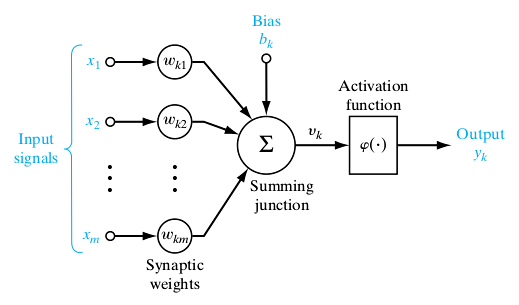
\includegraphics[width=0.9\linewidth]{figures/neuron.png} \\
    Source:~\cite{Haykin/2009}
\end{figure}

At the core of a neural network are individual artificial neurons, illustrated in Figure~\ref{fig:neuron}. A neuron consists of three main components: input signals, weights, and an activation function. Each neuron receives input from the previous layer or directly from the input data. These inputs are weighted, representing the importance of each input, and combined with a bias term. The result value are then passed through an activation function, which introduces non-linearity and determines the output of the neuron. One example of an activation function is the Rectified Linear Unit (ReLU) activation, which returns the input if it is positive and zero otherwise.

Neurons are combined to form layers in a neural network. Each layer serves a specific purpose in processing and transforming the input data. The input layer directly receives the input data and passes it to the subsequent layers. The hidden layers, located between the input and output layers, are responsible for extracting and learning higher-level features from the input. These hidden layers enable the network to capture complex patterns and relationships within the data. Finally, the output layer produces the prediction for the given input. A specific type of neural network called a feedforward neural network (FNN) operates by allowing information to flow in one direction, from the input layer through the hidden layers to the output layer. When a neural network has multiple hidden layers, it is referred to as a deep neural network.

The learning process involves adjusting the network's parameters, such as weights and biases, to minimize the error between its predictions and the true values of the training samples. This adjustment is typically performed using an optimization algorithm to minimize a specified loss function. One commonly used loss function is the Mean Squared Error (MSE) loss function, which quantifies the error by calculating the average squared difference between the predicted and true values. For a more comprehensive understanding of the weight adjustment and training process in neural networks, Haykin (\citeyear{Haykin/2009}) provides in-depth insights.

To efficiently update the parameters, training is often performed on batches of data rather than individual samples. The batch size determines the number of training examples that are processed together before updating the network's parameters. Larger batch sizes can lead to more stable updates but require more memory and computation, while smaller batch sizes may result in more frequent updates but with higher variance.

By iteratively adjusting its parameters based on the training data, a neural network gradually improves its ability to make accurate predictions. The quality of the neural network heavily relies on the quality and diversity of the training samples used during the learning process. Additionally, the network's capacity to learn and generalize from the training data is influenced by its structural characteristics. A well-designed and appropriately structured neural network enhances learning efficiency and improves its ability to handle complex patterns and relationships within the data.

\subsection{Residual Networks}
\label{sec:background_resnets}

ResNet, short for Residual Network, was proposed by He et al.~(\citeyear{He.etal/2016}) and has gained significant attention due to its ability to address the vanishing gradient problem~\cite{Hochreiter/1998} and improve training performance for deep neural networks. While its initial success was in the field of image recognition, ResNet has also been investigated in the context of planning~\cite{Agostinelli.etal/2019,Ferber.etal/2022} as a means to address training deep neural networks.

ResNet introduces the concept of residual connections or skip connections, which enable the network to learn residual mappings. These connections allow the network to bypass certain layers and pass the input directly to deeper layers. By doing so, ResNet mitigates the degradation problem that can occur in very deep networks, where adding more layers leads to decreased accuracy. The residual connections help preserve information and facilitate the flow of gradients during the training process.

\begin{figure}[ht]
    \caption[A regular block and a residual block.]{A regular block (left) and a residual block (right).}
    \label{fig:residual_block}
    \addvspace{\baselineskip}
    \centering
    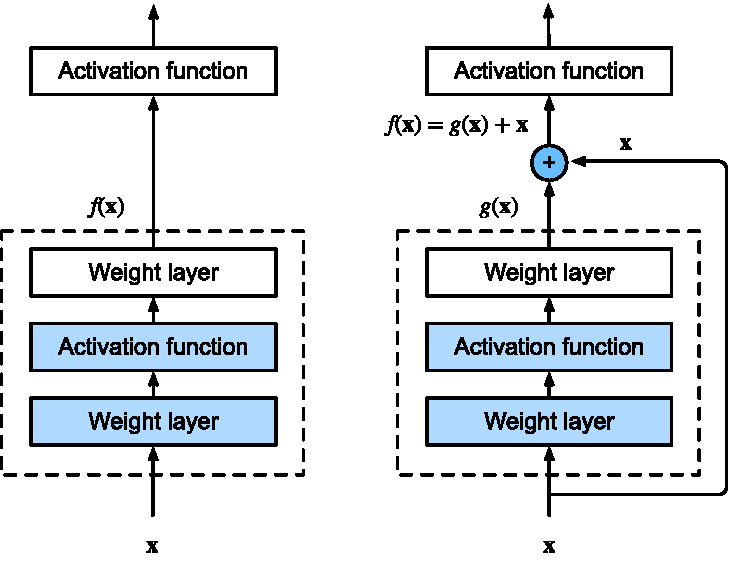
\includegraphics[width=0.75\linewidth]{figures/residual_block.pdf} \\
    Source:~\cite{Zhang.etal/2021}
\end{figure}

The Figure~\ref{fig:residual_block} illustrates a schematic representation of both a regular block and a residual block, with a shortcut connection that skips one layer, in a ResNet architecture. In a regular block, the output of its layers is directly mapped to the activation function. On the other hand, in a residual block, the network needs to learn the residual mapping $g(x)=f(x)-x$, making it easier for the network to optimize the model's performance. He et al.~(\citeyear{He.etal/2016}) provides a more detailed understanding of the ResNets.

\subsection{Learning Heuristic Functions}
\label{sec:background_learningheuristics}

Many heuristics for classical planning are derived from a model of the task, such as the \sas model introduced in this chapter. An obvious alternative is to learn to map a state $s$ to its heuristic value $h(s)$. We focus here on learning with NNs, although other supervised learning methods could be used. To learn a heuristic function, an NN is trained on pairs of states~$s$ and cost-to-goal estimates~$c$. The learned heuristic functions are usually not admissible, so traditional optimality guarantees are lost.

A propositional representation of a state is more suitable for learning functions over states. To this end, consider a planning task $\Pi=\langle\mathcal{V},\mathcal{O},s_0,s^*, \text{cost}\rangle$, and let $\mathcal{V}=\{v_1,\ldots,v_n\}$ and $D(v_i)=\{d_{i1},\ldots,d_{i,s_i}\}$, $i\in[n]$ be some order of the variables and their domains. We represent any state $s$ by a sequence of facts $$\mathcal{F}(s)=(f_{11},f_{12},\ldots,f_{1,s_1},\ldots,f_{n1},f_{n2},\ldots,f_{n,s_n}),$$ where each fact $f_{ij}=[s(v_i)=d_{ij}]$ indicates if variable $v_i$ assumes value $d_{ij}$ in state $s$. Note that facts $\mathcal{F}_i=\{f_{i1},\ldots,f_{i,s_i}\}$ corresponding to variable $v_i$ satisfy the consistency condition $\sum_{f\in \mathcal{F}_i} f\leq 1$ since each variable assumes at most one value, and $\sum_{f\in \mathcal{F}_i} f=0$ only if $v_i$ is undefined. More generally, for any set of facts $\mathcal{F}$ we write $\mutex(\mathcal{F})$ if $\sum_{f\in \mathcal{F}} [f]\leq 1$ must be satisfied in states of $\Pi$. Many planning systems can deduce mutexes from the description of the planning task $\Pi$~\cite{Helmert/2009}; we will discuss and analyze their utility for sampling states later. Some architectures provide additional input to the NN, e.g.,~the propositional representation of the goal condition. The target output for training may be the cost-to-goal estimates directly or some encoding of them.

An important aspect of sample generation related to challenges C1 and C2 (Section \ref{sec:intro}) is the degree of dependency on the domain model -- ideally, we would like to learn in a model-free setting -- or the planning task and the cost of generating the samples. The cost of sample generation depends on the number of samples and the cost to generate each. This generates the problem of deciding how many samples are required, although in general, only a very small part of the state space can be sampled. More importantly, ideal samples would be labeled with the perfect heuristic $h^*$, which maps each state~$s$ to the cost of an optimal $s$-plan or $\infty$ if no such plan exists. In general, ideal labeling is impractical since it requires solving the planning task on a large number of initial states. Therefore, we are mainly interested in good heuristic estimates that can be generated fast. We analyze the influence of sample size and quality experimentally later.

Additionally, and related to challenges C3 and C4, network architecture and sample generation depends on the range of tasks the learner intends to generalize. This may be the state space of a planning task, a planning domain, or an entire planning formalism. In the first case, the set of planning tasks is defined over any pair of initial state $s_0$ and goal $s^*$. Often the set of planning tasks is restricted to select the initial state from the \fssp of some given initial state and to a fixed goal. In the second case, the learned function has to generalize over all domain tasks. Finally, a learning-based heuristic that generalizes over a planning formalism is domain-independent. An important aspect of sample generation is the distribution of states part of the sample set. For example, the sample set can contain only states with a short distance to the goal or only states with a short distance to the initial states. In this dissertation, the distribution of states describes how often each \hstar-value occurs in the sample set.

\section{Related Work}
\label{sec:background_relatedwork}

There have been two main research foci on learning heuristic functions. The first uses strongly model-based approaches to generate samples and aims to generalize over domains or a planning formalism. The second uses partially model-based approaches to generate samples and aims to generalize only over a state space. We describe these approaches as partially model-based since they only use the model to identify mutexes.

\subsection{Strongly Model-Based}

The usual setting for the first set of approaches~\cite{Toyer.etal/2018,Shen.etal/2020,Toyer.etal/2020,Gehring.etal/2022,Stahlberg.etal/2022} is to train a structured NN with samples of small tasks of a domain generated with a strongly model-based method and evaluated on larger tasks of the same domain. Structured networks trained can be general networks such as neural logic machines~\cite{Dong.etal/2018} and graph neural networks~\cite{Gori.etal/2005,Scarselli.etal/2008}

In the context of planning, Shen et al.~(\citeyear{Shen.etal/2020}) introduced hypergraph neural networks (HGN) as an extension of graph networks~\cite{Battaglia.etal/2018}. HGN aims to learn planning heuristics through training, with a particular focus on developing domain-independent heuristics capable of generalizing across various domains, as well as domain-specific and multi-domain heuristics. A HGN encompasses vertices representing task propositions within a hypergraph structure, with edges denoting actions connecting the preconditions to their effects. The network learns latent features directly from the hypergraph representation of the planning problem.

Another approach proposed explicitly for planning tasks is the Action Schema Networks~(ASNet)~\cite{Toyer.etal/2018}. ASNets are composed of alternating proposition and action layers, with the first and last always being an action layer. Each action layer contains an action module for each action in a specific task, while each propositional layer contains a proposition module for each proposition in the task. Weight sharing is employed to optimize efficiency, where action modules with actions derived from the same action schema share the same weight, and proposition modules with propositions derived from the same predicate share the same weight. This weight sharing allows for the reuse of a single set of learned weights across all tasks within a class of planning problems.

These networks require the logical description of the domain and the task to be instantiated and can generalize well, with competitive results compared to logic-based heuristics. These approaches also help in understanding learning heuristics. For example, the main goal of St\aa hlberg et al.~(\citeyear{Stahlberg.etal/2022}) is to understand the expressive power and limitations of learning heuristics. The main limitation of these approaches is the strong dependence on the domain model and task description.

\subsection{Partially Model-Based}

The second set of approaches~\cite{Ferber.etal/2020a, Yu.etal/2020, Ferber.etal/2022, OToole/2022} typically trains an FNN and evaluates the learned heuristic on a state space using tasks with the same goal and different initial states. These networks are trained with pairs of states and cost-to-goal estimates. In this setting, Ferber et al.~(\citeyear{Ferber.etal/2020a}) systematically study hyperparameters on the architecture of the FNN and found that their influence is secondary. They found that for a fixed architecture, two aspects significantly influence how informed the heuristic is: the subset of selected samples and the size of the sample set. 

Ferber et al.~(\citeyear{Ferber.etal/2022}) uses a combination of backward and forward searches~\cite{Arfaee.etal/2011}. First, it generates new initial states with backward random walks and then solves them with a GBFS guided by a learned heuristic. The sampling is performed in parallel with the training, and the number of samples per search varies throughout the process. Initially, it starts with a random value ranging from $0$ to $5$, and doubles as plans are found. The plans found provide the samples for the next training epoch, where each sample is a state in a plan with the cost-to-goal estimate as its distance to the goal through the plan. Their FNN architecture is a ResNet with two hidden layers and a residual block consisting of two more hidden layers.

O'Toole et al.~(\citeyear{OToole/2022}) uses the same FNN architecture as Ferber et al.~(\citeyear{Ferber.etal/2022}), which is also applied in this dissertation. They employ random walks to perform $5$ backward searches from the goal, with a depth of $500$, where the depth at which the state is generated serves as a cost-to-goal estimate. Each sampled partial state is then converted into $20$ complete states and added to the sample set. Furthermore, they sample an additional $50$\,K randomly generated states with high cost-to-goal estimates, resulting in a total of $100$\,K samples. They showed that random sampling significantly improves the performance of the heuristic function.

Yu et al.~(\citeyear{Yu.etal/2020}) employed a backward search approach using the DFS algorithm. In their best configuration, they perform $800$ searches, sampling $500$ states each. Thus, their sample set comprises $400$\,K states, with the depth at which each state was generated serving as a cost-to-goal estimate. In contrast to the previous approaches, they use a compact FNN consisting of only one hidden layer with $16$ neurons.

The methods from the partially model-based approaches are highly independent of the domain model and planning task description and require low computational resources to generate samples and train the FNN. However, they suffer from high performance variability, given the FNN initialization and the sample set used. Also, despite having competitive results compared to logic-based heuristics, they are still unable to surpass the goal-count heuristic.

\chapter{Sample Generation}
\label{sec:sampling}

\rvi{WIP from here until the end of the chapter}

We aim to investigate sample generation systematically. Therefore, we focus on how three aspects of sample generation influence the performance of the learned heuristic to guide a search algorithm: the distribution of states $s_i$ in the state space part of the sample set, the quality of the estimates $h_i$ of samples with respect to the $\hstar$-value, and the methods that generate sample sets. In our setting, learning a heuristic function requires a set of samples $(s_1,h_1),\ldots,(s_N,h_N)$, where each sample $(s_i,h_i), i\in[N]$ consists of a state $s_i$ and a cost-to-goal estimate (or $h$-value) $h_i$.

We restrict our study to generalizing over planning tasks with initial states part of the same forward state space~(\fssp) and a fixed goal condition. We study model-free approaches with access to predecessors and successors of partial states through a black-box function, the goal condition, and the domain of each variable. We also study model-based approaches that have access to mutexes derived from a \sas model. We approach first, in Section~\ref{sec:generation}, the generation of states, and then, in Section~\ref{sec:hvalue}, the estimation of the cost-to-goal. In both sections, we discuss approaches from the literature and introduce new methods. The new methods are a novel sampling strategy combining regression by breadth-first search with random walk, an adaptive regression limit, and two improvement methods for cost-to-goal estimates.

\section{Generation of States}
\label{sec:generation}

Unlike other domains in machine learning, where datasets of samples are often collected in real-world experiments and need to be manually annotated and curated, sample generation here is an algorithmic problem since we have access to the state space and can compute cost-to-goal estimates. Approaches from the literature to generate the states include methods based on progression from one or more initial states, random sampling of the state space, or regression from the goal. In both progression and regression, one can apply different expansion strategies such as random walks, breadth- or depth-first searches, or teacher searches which include ``on policy'' searches in methods using reinforcement learning or bootstrapping~\cite{Arfaee.etal/2011}. A problem in progression and random sampling is obtaining the cost-to-goal estimates. Without access to efficiently computable heuristic functions, or in model-free approaches, these values have to be obtained by search, which can have a cost exponential in the size of the task. To remain less dependent on models than logic-based methods and also more general, we focus on regression for which an upper bound on the cost-to-goal is readily available, discussed in Sections~\ref{sec:sampling-generation}~and~\ref{sec:rollout-depth-limit}. Still, regression leads to partial states, so the problem of generating complete states is addressed in Section~\ref{sec:sample-completion}. Random sampling is also discussed in Section~\ref{sec:random-samples-theory}.

\subsection{Sampling by Regression}
\label{sec:sampling-generation}

To generate samples, we expand the backward state space through regression. We consider expansion by breadth-first search (\bfs) and depth-first search (\dfs), by random walks (\rw), as well as a combination of BFS with random walks explained below. A regression rollout is defined as a series of state expansions, and it stops if the last expanded state has no predecessors or is at the depth limit $L$. The sampling generation process stops if the number of required samples $N$ has been reached. Note that random walks can have multiple rollouts due to $L$, while \bfs and \dfs only have one -- except if the number of states in the backward state space is less than $N$, in which case they need to perform more than one rollout.

During expansion, we optionally use mutexes obtained from an analysis of the planning task -- in our case as computed by Fast Downward~\cite{Helmert/2006} -- to discard partial states which cannot be completed to complete states without violating a mutex, as described in Section~\ref{sec:sample-completion}. We also discard repeated partial states for random walk rollouts, such that a single rollout never cycles, although the same partial state may be sampled several times in different rollouts. Starting from $h(s^*)=0$, a state $s'\in\pred(s,o)$ obtained by applying an operator $o$ backwards to state $s$ has a cost-to-goal estimate $h(s')=h(s)+\text{cost}(o)$. We reset to $h(s)=0$ the cost-to-goal estimate for samples $s\subseteq s^*$ that satisfy the goal condition. States are added to the sample set when generated in the random walks and when expanded in BFS and DFS. In all methods, operators backward applicable to a state are applied in random order.

Different expansion strategies generate sample sets with varying frequencies of  optimal distances from the goal. In our experience, good coverage of states close to the goal, such as those obtained by BFS or random walks, is useful, as is the greater depth obtained by DFS or random walks. However, random walks from the goal often sample states close to the goal multiple times, and DFS can lead to a concentration of distant samples from the goal. Based on these observations, we propose a novel combination of BFS and random walks called \bfsrw that aims to have a good coverage close to the goal and a diverse set of samples from the remaining state space. \bfsrw has two phases. In the first phase, a fixed percentage $p_\bfsrw$ of the $N$ samples is generated by BFS. (Note that $p_\bfsrw$ can additionally represent time and memory limitations -- in this case, \bfs stops once either of them is reached first.) The \bfs expands a state from layer $k$ that generates $n$ states from layer $k+1$, and these states are sampled only if the current total samples plus $n$ are within $p_{\bfsrw}N$ samples; otherwise, no states are sampled and \bfs expands another state. Let $Q$ be the states of the set of samples that have not been expanded. The second phase generates multiple random walk rollouts, each starting from a state in $Q$ chosen randomly with a complete replacement only after all states have been selected once. This is repeated until reaching $N$ samples in the sample set. During a random walk, states sampled in the BFS phase are discarded.

\subsection{Maximum Regression Limit}
\label{sec:rollout-depth-limit}

A simple strategy to limit the expansion depth is to define some maximum limit $L$. This has been used in previous work, e.g.,~by \citeyear{Yu.etal/2020} and \citeyear{OToole/2022} with $L=200$ and $L=500$, respectively. A fixed limit is not the optimal choice for tasks with state spaces of different diameters or different maximum distances to a fixed goal when we aim for a representative sample of the state space. This is a problem in particular for regression: if the maximum regression limit $L$ overestimates the maximum distance-to-goal by much, the corresponding cost-to-goal estimates will be too large; if it underestimates it, samples may be concentrated too close to the goal.

Therefore, the most effective maximum regression limit for a fixed goal should be defined as a function of the longest distance \distfarthest from the goal state to any other potential initial state. For BFS, \distfarthest would be the ideal estimate; for DFS and random walks, higher limits are required since they do not follow the shortest paths. Since \distfarthest, in general, is unknown, we propose to define a maximum regression limit $L$ by two adaptive, approximated methods, according to the input task parameters, the first of which is model-free and the second model-based. The first is a regression limit that equals the number of facts $L=F=|\mathcal{F}(s_0)|$. The second is to set $L=\bar F=\ceil{\facts/\overline{\eff}}$ where $\overline{\eff}=\sum_{o\in \mathcal{O}} |\eff(o)|/|\mathcal{O}|$, i.e.,~the number of facts per mean number of effects in the operators.

\subsection{Sample Completion}
\label{sec:sample-completion}

Regression sampling generates a set of partial states, while the NN is trained on and receives as input complete states during the search. Each partial state can be completed by assigning a value $s(v)\in\dom(v)$ to all fact pairs $(v,s(v))$ where $s(v)=\bot$. Since it makes no assumptions except the domains, we consider this strategy model-free. We further study two stronger methods of generating complete states: a model-based one that uses mutexes and an ideal completion that only generates states that are reachable from the initial states of interest.

The model-based method also assigns a random value $s(v)\in\dom(v)$ to each undefined variable but excludes states that do not satisfy mutexes derived from the planning task. This is achieved by rejection sampling, where the undefined variables are processed in random order and set to a random value that does not violate the mutexes. If the state could not be completed in $10$\,K trial orders, we leave the facts undefined, i.e., set to false (zero)\footnote{Empirically this case is negligible since it occurs in about $0.1\,\%$ of the samples, in four of nine domains.}.

The model-based solution can still generate states that can never be reached during the search. To study the effect of generating only relevant states, we therefore also include an ideal state completion method. This method applies only to small tasks, where we can enumerate the complete forward state space \fssp of the initial state $s_0$. Then, to complete a partial state $s$ we sample a random state from $s~\cap$~\fssp. Since we sample by regression for some states $s~\cap$~\fssp may be empty; such states are discarded during regression.

\subsection{Randomly Generated Samples}
\label{sec:random-samples-theory}

\citeyear{OToole/2022} have shown that adding randomly generated samples to a set of samples generated by expansion improves the performance of the search algorithm guided by the learned heuristic. They propose to set the cost-to-goal estimate for randomly generated samples to $L+1$ for a maximum regression limit of $L$. To study the effect of randomly generated samples, we include this method in our study. These samples are generated from fully undefined states using the model-based technique described in the previous section. If the generated state $s$ is already part of the sample set, i.e.,~$s = s_i$ for some $i\in[N]$ it receives cost-to-goal estimate $h_i$, otherwise the cost estimate $1+\max_{i\in[N]} h_i$ that is larger than all samples estimates. For simplicity, from this point on we refer to ``randomly generated samples'' as ``random samples''.

\section{Improving Cost-to-Goal Estimates}
\label{sec:hvalue}

We start by observing that cost-to-goal estimates never underestimate the true cost-to-goal $h^{*}$, as follows.

\begin{property}
    \label{prop:hvalue}
    The cost-to-goal estimate $h(s)$ of a sample $s$ obtained by regression satisfies $h(s)\geq h^*(s)$.
\end{property}
\begin{proof}
    This follows simply because each estimate is witnessed by a plan. As observed in Section~\ref{sec:background}, a valid regression sequence $\rho=(o_1,\ldots,o_k)$ generates a sequence of partial states that can reach the goal in at most $k$ steps and with cost at most $\sum_{i\in[k]}\text{cost}(o_i)$, which cannot be lower than the optimal cost.
\end{proof}

In general, we expect better $h$-value estimates to lead to better-learned heuristics, and in turn to less expanded states during a search, although this is not necessarily the case \cite{Holte/2010}. Therefore, we apply two simple procedures that improve the cost-to-goal estimates but maintain \cref{prop:hvalue}. The first, dubbed \hmin, minimizes estimates over repeated samples, and the second, \hvfc, over successors of samples.

\subsection{Improvement of Repeated Samples}
\label{sec:hmin}

In most state spaces, it is common for a state to be sampled in more than one random walk rollout, ending up with multiple duplicates with different estimates. Thus, for all sampled states $s$ we update each cost-to-goal estimate to the best estimate $h(s) = \min\{h_i \mid s=s_i, i\in[N]\}$. Since different partial states can generate identical complete states, the improvement is applied to partial states as well as complete states. We call this procedure \emph{sample improvement} (\hmin). Choosing the minimum $h$-value is clearly sound since, in all cases, we have valid plans from a regression that witness these distances; for the same reason, \cref{prop:hvalue} still holds.

\subsection{Improvement over Successors}
\label{sec:hvfc}

Besides sampling the same states, it is common to sample states that are neighbors in the state space, particularly for states close to the goal. This can be used to improve the cost-to-goal estimates, as follows. Consider a directed graph $G=(V,A)$ over all sampled partial states, i.e.,~$V=\{s_i\mid i\in[N]\}$. For every pair of states $s,t\in V$ such that for some operator $o\in\mathcal{O}$ applicable to $s$ we have $\sucs(s,o)\subseteq t$, we add an arc $(s,t)$ of length $\text{cost}(o)$ to $A$. (Unlike in regression, if $\pre(o)$ mentions an undefined variable in $s$ then $o$ is not applicable.) For fast subset, we keep all samples in a trie and search for each successor in the states that are supersets. For partial states generated by regression, by construction, at least one such successor exists, except for the goal state $s^*$. We then compute the shortest paths to the goal in graph $G$ (e.g.,~via the Dijkstra algorithm), and update the cost-to-goal estimates with these distances. We call this procedure \emph{successor improvement} (\hvfc). As for \hmin, all distances are witnessed by plans, so \cref{prop:hvalue} is maintained.

\section{Example}
\label{sec:example}

%Check the example of Fukunaga. We need: a small example that is able to demonstrate all techniques: regression, partial states, minimization, \bfs, random walks, etc.

\chapter{Experiments}
\label{sec:experiments}

In this section, we present two sets of experiments. In the first set, we analyze the behavior of sampling methods on planning tasks for which we can enumerate the complete state space with associated perfect cost-to-goal estimates \hstar. We study how different techniques can influence the number of state expansions by a search algorithm. In the second set, we evaluate how our findings generalize to a practical setting with large planning tasks. Our methods are then compared to logic-based heuristics.

\section{Settings}
\label{sec:settings}

We use a residual neural network~\cite{he2016deep} to learn a heuristic for a state space. The network's input is a Boolean representation of the states, where a fact is set to~$1$ if it is true in the state and~$0$ otherwise, as explained in \cref{sec:learning-heuristics}, and its output is a single neuron with the predicted \h-value. The network has two hidden layers followed by a residual block with two hidden layers. Each hidden layer has~$250$ neurons that use ReLU activation and are initialized as proposed by \citet{he2015delving}. The training uses the Adam optimizer~\cite{kingma2015adam}, learning rate of~$10^{-4}$, early-stop patience of~$100$, and MSE loss function. Due to better results in preliminary experiments, we use batch sizes of~$64$ for small and~$512$ for large state spaces. We use $90\,\%$ of the sampled data as the training set, with the remaining $10\,\%$ as the validation set. In the experiments, different learned heuristics are denoted as~$\hat h_A$, where~$A$ indicates different algorithmic choices.

We select the domains and tasks from \citet{ferber2022neural}: Blocks, Depot, Grid, N-Puzzle, Pipes-NT, Rovers, Scanalyzer, Storage, Transport, and VisitAll. All domains have unit costs except for Scanalyzer and Transport, for which we consider the variant with unit costs. All methods are implemented on the Neural~Fast~Downward planning system with PyTorch~1.9.0~\cite{ferber2020neural,paszke2019pytorch}. Our source code, planning tasks, and experiments are available\footnote{Available at \url{https://github.com/bettker/NeuralFastDownward}}. All experiments were run on a PC with an AMD~Ryzen~9~3900X processor, using a single core with $4$\,GB RAM per process. We solve all tasks with \gbfs guided by the heuristic~\h with the lowest generation order as a tie-breaking strategy.

We note that an NN may fail to train if, after initialization, it outputs zero for all training samples~(this is called ``born dead'' in \citet{lu2020dying}). This occurs with a non-negligible frequency in experiments on smaller state spaces with fewer samples. Thus, we test for this condition. Suppose the network outputs zero for all samples in the training set after initialization. In that case, we reinitialize with a different seed until the network outputs a non-zero value for some sample.

We propose a baseline \hnnbase to establish a point of comparison for evaluating the performance of the approaches. The baseline refers to a NN configured similarly to previous sample-based methods described in \cref{sec:related-work-sample-based}. The \hnnbase is trained using random walks with $L=200$. Mutexes are applied during the regression and for state completion, but resetting the \h-value to~$0$ in goal states and the improvement strategies SAI and SUI are turned off. By comparing the results of our approaches with the baseline, we can assess the potential improvements over existing methods.

To determine a value for $p_{\bfsrw}$, preliminary experiments in small state spaces were performed using $p_{\bfsrw}\in\{0.01,0.05,0.1,0.2,\ldots,0.9\}$. We use the same baseline configuration but with the FSM sampling algorithm. The corresponding geometric mean expansions obtained were $84.92$, $79.51$, $74.05$, $79.46$, $80.39$, $80.79$, $96.17$, $120.42$, $133.99$, $167.14$, and $175.58$, respectively. As a result, we set a fixed value of $p_{\bfsrw} = 0.1$ for the experiments.

\section{Small State Spaces}
\label{sec:small-experiments}

In this section, we study the behavior of different sampling methods on small state spaces. For each domain, we select the task from the IPC benchmarks with the largest size state space that can be enumerated completely to obtain \hstar-values. We only select tasks with state spaces with $30$\,K~states or more, and fewer than $1$\,M~states. \cref{tab:small-fss-size} shows the tasks and their state space sizes. For domains Grid, Rovers, Scanalyzer, and Transport, the best task found had fewer than $30$\,K states, and VisitAll more than $1$\,M, so we manually modified these tasks. We could not find a task within our limits for Depot, Pipes-NT and Storage, so they were excluded from our experiments. We generate the initial states for the small state spaces by performing a random walk of length~$200$ from the original initial state of a task. Rovers, Scanalyzer, and VisitAll had duplicated initial states or states that satisfied a goal state. Thus, we generate the initial states for these domains with random walks of length~$25$, $50$, and $8$, respectively.

\begin{table}[tb]
    \caption[Size of the forward state spaces for the selected domains.]{Size of the forward state spaces for the selected small tasks in seven domains. Tasks marked with~$*$ were modified.} 
    \label{tab:small-fss-size}
    \addmargin
    \centering
    \begin{tabular}{llr|llr}
    Domain & Task & \#States & Domain & Task & \#States \\ 
    \midrule
    Blocks & blocks-7-0 & 65990 & Scanalyzer & p03$^*$ & 46080 \\
    Grid & prob01$^*$ & 452353 & Transport & p02$^*$ & 637632 \\
    N-Puzzle & prob-n3-1 & 181440 & VisitAll & p-1-4$^*$ & 79931 \\
    Rovers & p03$^*$ & 565824 & & & \\
\end{tabular}

\end{table}

In the small state space experiments, the coverage for all methods is $100\,\%$. Therefore we use the number of expanded states to evaluate the quality of the heuristic function. In these experiments, we report means over experiments with five different network seeds, five different sample seeds, and $50$~initial states. The training time has been limited to $30$~minutes. If not stated otherwise, methods \bfs, \dfs, \rw, and \bfsrw use mutexes, the improvement strategies SAI and SUI, and the number of samples is equal to $1\%$ of the state space size. After initialization, the percentage of networks that output~$0$ for all samples was at most $40\,\%$~(in Blocks), and all networks successfully passed the initialization test after the second initialization. Under these conditions, less than $1.5\,\%$ of the NNs did not converge within the time limit.

\subsection{Distribution of States}
\label{sec:small-exps-distribution}

Our first set of experiments aims to analyze the influence of the distribution of sampled states in the state space on the quality of the learned heuristics. We compare different sample generation algorithms, regression limits, random sample percentages, and state completion methods. If not stated otherwise, for the parameters that are not varied, we use the baseline setting defined above~(regression limit~$L=200$, mutexes, no cost-to-goal improvement methods).

\subsubsection{Sample Generation Algorithms}
\label{sec:small-exps-algorithm}

This experiment compares four sample generation algorithms: \bfs, \dfs, \rw, and \bfsrw. To control the effect of the cost-to-goal estimates on the quality of the learned heuristic, we replace sample estimates with perfect values~\hstar before training. \cref{tab:small-sampling-hstar} shows the number of expanded states of a \gbfs guided by the learned heuristics and the mean \hstar-values over the sampled states. We see that heuristic \hnnl{\bfs} leads to more expanded states than \hnnl{\dfs}, which in turn expands about $50\,\%$ more states than \hnnl{\rw} and \hnnl{\bfsrw}, which perform similarly. Using \hnnl{\bfs} is significantly worse and leads to the highest or close to the highest number of expansions in all domains. Heuristic \hnnl{\dfs} has a high number of expansions in Blocks, N-Puzzle, and Transport. Looking at the mean \hstar-values, we see that samples generated by \bfs have the lowest, and those by \dfs the highest mean estimates in all domains. Although the distribution of \dfs is closest to that of the whole state space~(inferred from the mean \hstar-values), the resulting heuristic expands more states than \rw and \bfsrw, which generate states closer to the goal. Therefore, multiple random walk rollouts seem better than a single rollout with \bfs or \dfs due to increased sample diversity in different portions of the state space, covering states more likely to be visited during the search.

\begin{table}[tb]
    \caption[Comparison of sampling strategies on \hstar-values.]{Comparison of sampling strategies~\bfs, \dfs, \rw, and \bfsrw on \hstar-values. Expanded states of \gbfs with learned heuristics and mean \hstar-values over the entire forward state space and the generated sample sets.}
    \label{tab:small-sampling-hstar}
    \addmargin
    \centering
    \begin{tabular}{lrrrrrrrrr}
    & \multicolumn{4}{c}{Expanded states} & \multicolumn{5}{c}{Mean \hstar-values} \\
    \cmidrule(lr){2-5}\cmidrule(lr){6-10}
    Domain & \hnnl{\bfs} & \hnnl{\dfs} & \hnnl{\rw} & \hnnl{\bfsrw} & FSS & \bfs & \dfs & \rw & \bfsrw \\
    \midrule
    Blocks & 5047.1 & 85.9 & 44.4 & \textbf{37.3} & 18.8 & 10.8 & 17.7 & 11.9 & 14.4 \\
    Grid & 112.7 & 122.4 & \textbf{99.2} & 110.3 & 16.6 & 5.3 & 17.1 & 7.2 & 8.9 \\
    N-Puzzle & 1477.2 & 176.8 & 109.5 & \textbf{109.2} & 22.0 & 10.4 & 20.2 & 20.0 & 19.8 \\
    Rovers & 12.9 & 13.1 & \textbf{11.8} & 11.8 & 6.4 & 2.3 & 5.2 & 5.0 & 5.0 \\
    Scanalyzer & 175.9 & 25.5 & \textbf{24.5} & 24.9 & 8.3 & 2.9 & 7.9 & 7.1 & 6.5 \\
    Transport & 135.1 & 45.0 & 19.6 & \textbf{19.2} & 12.2 & 2.9 & 11.3 & 10.0 & 9.5 \\
    VisitAll & 53.3 & 22.0 & 19.2 & \textbf{18.7} & 9.0 & 2.0 & 9.1 & 6.8 & 6.6 \\
    \midrule
    Geo.~mean & 201.9 & 48.3 & 34.0 & 33.5 & 12.2 & 4.2 & 11.4 & 8.8 & 9.1 \\
\end{tabular}

\end{table}

We now compare these results to results shown in \cref{tab:small-sampling-h}, obtained on exactly the same states but using the cost-to-goal estimates obtained during sampling for training the NN. Note that the results for \bfs with estimated costs to the goal differ from those with exact values in \cref{tab:small-sampling-hstar}. This happens because, during regression with \bfs, the cost-to-goal estimates are only exact on partial states; when turning them to complete states, the estimates can be larger than \hstar. Thus \hnnl{\bfs} with the estimates obtained during regression is less informed.

We can see that the relative order of the methods concerning the number of expanded states remains the same, although all methods expand more states. The increase in the number of expanded states is highest for \hnnl{\dfs}, which expands about seven times more states. In contrast, the other methods expand about twice as much, meaning that the estimates produced by \dfs during regression are inferior to those produced by the other methods. The mean \h-values confirm this: we can see that DFS significantly overestimates the true distances. Although \bfs has an estimation quality close to \hstar-value, its expanded states also degrade. These results suggest that sampling more states in localized regions of the state space~(\bfs closer to the goal and \dfs more distant) is insufficient to achieve good results during the search with \gbfs. Furthermore, \hnnl{\bfsrw} expands fewer states than \hnnl{\rw} and is the best in five of seven domains. Because \hnnl{\bfsrw} had a lower increase in expansions compared to \hnnl{\rw}, we focus on \bfsrw in the remaining experiments.

\begin{table}[tb]
    \caption[Comparison of sampling strategies on estimated \h-values.]{Comparison of sampling strategies \bfs, \dfs, \rw, and \bfsrw on estimated \h-values. Expanded states of \gbfs with learned heuristics and mean \h-values over the entire forward state space and the generated sample sets.}
    \label{tab:small-sampling-h}
    \addmargin
    \centering
    \begin{tabular}{lrrrrrrrrr}
    & \multicolumn{4}{c}{Expanded states} & \multicolumn{5}{c}{Mean \h-values} \\
    \cmidrule(lr){2-5}\cmidrule(lr){6-10}
    Domain & \hnnl{\bfs} & \hnnl{\dfs} & \hnnl{\rw} & \hnnl{\bfsrw} & FSS & \bfs & \dfs & \rw & \bfsrw \\
    \midrule
    Blocks & 5047.1 & 205.6 & 87.0 & \textbf{80.8} & 18.8 & 10.8 & 166.1 & 28.1 & 38.4 \\
    Grid & 431.2 & 4102.4 & \textbf{263.6} & 276.2 & 16.6 & 6.8 & 184.6 & 21.1 & 22.5 \\
    N-Puzzle & 1477.2 & 1092.5 & 237.6 & \textbf{177.1} & 22.0 & 10.4 & 187.5 & 96.3 & 90.6 \\
    Rovers & 91.8 & 27.8 & 21.9 & \textbf{18.8} & 6.4 & 4.6 & 27.1 & 25.9 & 24.9 \\
    Scanalyzer & 328.0 & 263.5 & 70.6 & \textbf{53.6} & 8.3 & 3.0 & 146.2 & 90.3 & 87.9 \\
    Transport & 215.1 & 1321.1 & \textbf{111.0} & 130.1 & 12.2 & 3.3 & 196.1 & 95.2 & 88.6 \\
    VisitAll & 170.4 & 44.6 & 22.0 & \textbf{21.5} & 9.0 & 2.7 & 28.5 & 22.5 & 22.4 \\ 
    \midrule
    Geo.~mean & 446.7 & 326.7 & 79.8 & 73.1 & 12.2 & 5.1 & 103.5 & 43.3 & 44.4 \\ 
\end{tabular}

\end{table}

\subsubsection{Maximum Regression Limit}
\label{sec:small-exps-rollout-limit}

In this experiment, we analyze the influence of the regression limit on the number of expanded states of sample generation strategy \bfsrw. We compare a fixed regression limit of~$L=200$ to setting the regression limit to the number of facts~\facts, or the number of facts divided by the mean number of effects~\meanfx. Values \facts and \meanfx for the selected tasks and the largest distance of any state from a goal state~\ssdiameter are shown in \cref{tab:small-rollout-limit}. Both \facts and \meanfx overestimate the largest distance \ssdiameter, except for \meanfx in three domains~(Blocks, Scanalyzer, and VisitAll). As discussed in \cref{sec:rollout-limit}, this is desirable since random walk rollouts do not follow the shortest paths.

\begin{table}[tb]
    \caption[State space information and expanded states with different regression limits.]{State space information and expanded states of \gbfs guided by \hnn trained on \bfsrw samples with different regression limits and no \h-value improvements. The value \ssdiameter is the distance of the state most distant from a goal state.}
    \label{tab:small-rollout-limit}
    \addmargin
    \centering
    \begin{tabular}{lrrrrrr}
    Domain & \ssdiameter & \facts & \meanfx & \rldefault & \rlfacts & \rlmeanfx \\
    \midrule
    Blocks & 24 & 64 & 17 & 80.76 & \textbf{58.06} & 185.00 \\
    Grid & 32 & 76 & 44 & 276.23 & 316.51 & \textbf{204.89} \\
    N-Puzzle & 31 & 81 & 41 & 177.12 & 104.52 & \textbf{80.83} \\
    Rovers & 19 & 32 & 27 & 18.85 & 17.74 & \textbf{16.50} \\
    Scanalyzer & 15 & 42 & 20 & \textbf{53.59} & 57.02 & 88.76 \\
    Transport & 17 & 66 & 35 & 130.14 & 82.35 & \textbf{58.13} \\
    VisitAll & 15 & 31 & 17 & \textbf{21.51} & 25.61 & 29.96 \\
    \midrule
    Geo.~mean & & & & 73.12 & 63.36 & 69.48 \\
\end{tabular}

\end{table}

The right-hand side of \cref{tab:small-rollout-limit} gives the number of expanded states for the three settings of $L$. We see that limits \facts and \meanfx perform better than the fixed limit~$200$, with \facts best on one, \meanfx on four, and $200$ on two tasks. Also, when a limit of~$200$ is best, \facts presents the closest results, but when \facts or \meanfx are best, a limit~$200$ can be much worse. Note that \facts is the best only in the domain where \meanfx underestimates \ssdiameter. To validate this, we set~$L=\ceil{c\bar F}$ for $c\in\{1.25,1.5,2,2.5,3,3.5\}$ in an additional experiment on domain Blocks. The number of expanded states decreases to~$c=3$ with a mean of $52.31$ expansions. Overall, the adaptive limits \facts and \meanfx are better estimates of the best regression limit.

\subsubsection{Randomly Generated Samples}
\label{sec:small-exps-random-samples}

In this experiment, we evaluate the effect of adding randomly generated samples to the sample set, as explained in \cref{sec:random-samples}. We generate sample sets~$S=\{(s_1,h_1),\ldots,(s_N,h_N)\}$ where $10\,\%, 20\,\%,\ldots,100\,\%$ are random samples~(to which the improvement strategies SAI and SUI are not applied) and the rest is sampled with \bfsrw and a regression limit~\meanfx. Random samples get an \h-value of~$H+1$ where $H=\max_{i\in[N]} h_i$ is the largest \h-value in samples~$S$, except when they are part of the samples, in which case they receive the corresponding estimate~(this happens in fewer than $1\,\%$ of the states). Note that when using $100\,\%$ of random samples, each has the cost-to-goal estimate equal to the regression limit~$L+1$ instead of~$H+1$, as we do not have samples in~$S$.

\begin{table}[tb]
    \caption[Expanded states from a varying percentage of randomly generated samples.]{Expanded states of \gbfs with a learned heuristic over samples generated by \bfsrw with regression limit~\meanfx, all cost-to-goal improvement strategies, and a varying percentage of randomly generated samples.}
    \label{tab:small-random-samples}
    \addmargin
    \centering
    \begin{tabular}{lrrrrrrrr}
    & \multicolumn{8}{c}{Percentage of random samples} \\
    \cmidrule(lr){2-9}
    Domain & 0 & 10 & 20 & 30 & 40 & 50 & 60 & 70 \\
    \midrule
    Blocks & 177.88 & 59.23 & 57.00 & 63.75 & 63.25 & \textbf{48.99} & 65.26 & 74.47 \\
    Grid & 124.89 & \textbf{60.77} & 66.52 & 79.81 & 64.33 & 66.87 & 75.92 & 115.44 \\
    N-Puzzle & 89.47 & 87.60 & \textbf{80.93} & 88.76 & 86.64 & 81.62 & 89.38 & 96.26 \\
    Rovers & 17.03 & 14.16 & \textbf{13.45} & 13.63 & 13.60 & 14.34 & 14.23 & 16.38 \\
    Scanalyzer & 55.29 & 37.88 & \textbf{28.34} & 33.74 & 32.37 & 42.94 & 28.85 & 35.83 \\
    Transport & \textbf{22.90} & 24.58 & 25.95 & 27.44 & 33.02 & 34.53 & 43.36 & 52.36 \\
    VisitAll & 30.90 & 22.70 & \textbf{21.78} & 22.05 & 22.11 & 23.11 & 24.45 & 25.75 \\
    \midrule
    Geo.~mean & 53.91 & 36.97 & 35.13 & 38.51 & 37.95 & 38.76 & 40.94 & 48.75 \\
\end{tabular}

\end{table}

\cref{tab:small-random-samples} shows the performance up to~$70\,\%$ random samples. We have omitted $80\,\%$, $90\,\%$, and $100\,\%$ since expansions are higher~(respectively $56.10$, $73.94$, and $11397.79$). The number of expansions is considerably reduced when using random samples, with $20\,\%$~random samples performing slightly better than other percentages. This also holds for individual domains, except Transport which expands on average a few states more, and N-Puzzle and Rovers, which expand a few states less.

To better understand the effect of random samples, we have performed three additional experiments with $20\,\%$ of random samples. The first focuses on cost-to-goal estimates. We keep the samples but replace $H+1$ with small values: a random \h-value from the sample set~$S$ or a random value drawn from $U[1,5]$. This leads to overall means of $295.65$ and $3832.14$ expanded states, respectively. The second experiment changes the distribution of the random samples: we force them to be part of the FSS. This leads to a mean of $36.90$ expanded states. Finally, the third experiment does not apply mutexes, leading to a mean of $36.11$ expanded states. From these additional experiments, it is clear that the most relevant factor is a high \h-value, and the distribution and quality of the states seem to matter less. Overall, the most probable explanation for the effect of random samples is that they help to increase the probability that the search is guided towards samples for which the network has learned good estimates, i.e.,~the samples obtained through regression.

\subsubsection{State Completion}
\label{sec:small-exps-state-completion}

Now we focus on how sampled partial states are converted to complete states. In this experiment, all the samples have perfect cost-to-goal estimates~\hstar. We compare three different state completion strategies for a partial state~$s$. All of them select a random state from the set of states represented by $s$ or a restriction of it: the set equals either to all states in~$s$~(no restrictions), only those states that satisfy mutexes, or only states from the forward state space~(perfect baseline).

\cref{tab:small-state-completion} presents the expanded states for these approaches. We can see that applying mutexes has a moderate effect and is very close to an ideal completion of the states. However, completing randomly also presents competitive results, except for N-Puzzle. Also, N-Puzzle with both restrictions should have similar results, as for this particular domain, all partial states completed respecting the mutexes are part of the FSS, but this is not the case due to noisy training (detailed in \cref{sec:noisy-training}). To confirm this, we ran $900$ experiments~, with $30$~sample seeds and $30$~network seeds, for N-Puzzle ``Mutex'' and ``FSS'', and we achieved similar mean expansions of $84.4$ and $88.66$, respectively.

\begin{table}[tb]
    \caption[Expanded states from different state completion approaches.]{Expanded states of \gbfs with \hnn trained with \bfsrw, \rlmeanfx, \hstar cost-to-goal estimates, and different state completion approaches.}
    \label{tab:small-state-completion}
    \addmargin
    \centering
    \begin{tabular}{lrrr}
    & \multicolumn{3}{c}{Restriction} \\
    \cmidrule(lr){2-4}
    Domain & None & Mutex & FSS \\
    \midrule
    Blocks & 212.30 & 207.18 & \textbf{190.96} \\
    Grid & 104.34 & 96.02 & \textbf{87.80} \\
    N-Puzzle & 225.62 & \textbf{79.42} & 98.71 \\
    Rovers & 11.50 & 11.74 & \textbf{10.65} \\
    Scanalyzer & \textbf{41.20} & 43.98 & 44.61 \\
    Transport & 17.98 & 17.86 & \textbf{16.65} \\
    VisitAll & \textbf{22.17} & 22.44 & 22.78 \\ 
    \midrule
    Geo.~mean & 51.37 & 44.15 & 43.57 \\ 
\end{tabular}

\end{table}

\subsection{Estimates of Cost-to-Goal}
\label{sec:small-exps-hvalue}

Our second set of experiments aims to analyze how techniques used to improve cost-to-goal estimates influence sample quality. To this end, we directly compare the difference of the improved estimates to \hstar-values. Then, to see how well the learned heuristics generalize, we evaluate them over the forward state spaces from \cref{tab:small-fss-size}.

\subsubsection{Quality of Estimates}
\label{sec:small-exps-hvalue-quality}

First, we compare the quality of the cost-to-goal estimates to \hstar with and without \h-value~improvement techniques and distinct regression limits, as shown in \cref{tab:small-difference-hstar}. This table shows the mean absolute difference between the sample estimates and \hstar, so smaller means indicate better approximations. Note that we are not evaluating an NN's output but the sample set's cost-to-goal estimates.

\begin{table}[tb]
    \caption[Mean difference of the cost-to-goal estimates to \hstar.]{Mean difference of the cost-to-goal estimates of samples of the sample set to \hstar.}
    \label{tab:small-difference-hstar}
    \addmargin
    \centering
    \begin{tabular}{lrrrrrrr}
    & \multicolumn{3}{c}{No improvements} & \multicolumn{4}{c}{With SAI and SUI} \\
    \cmidrule(lr){2-4}\cmidrule(lr){5-8}
    Domain & \rldefault & \rlfacts & \rlmeanfx & \rldefault & \rlfacts & \rlmeanfx \\
    \midrule
    Blocks & 24.01 & 12.90 & 0.91 & 12.56 & 6.90 & \textbf{0.18} \\
    Grid & 13.60 & 13.29 & 9.84 & 1.32 & 1.32 & \textbf{0.61} \\
    N-Puzzle & 70.87 & 21.80 & 6.10 & 60.79 & 19.18 & \textbf{5.11} \\
    Rovers & 19.92 & 11.58 & 9.74 & 6.70 & 5.29 & \textbf{4.88} \\
    Scanalyzer & 81.35 & 15.07 & 6.09 & 20.16 & 5.59 & \textbf{1.89} \\
    Transport & 79.06 & 23.42 & 10.98 & 24.59 & 5.98 & \textbf{2.44} \\
    VisitAll & 15.80 & 9.07 & 4.58 & 5.64 & 4.06 & \textbf{2.15} \\
    \midrule
    Geo.~mean & 33.45 & 14.56 & 5.56 & 10.95 & 5.35 & 1.60 \\
\end{tabular}

\end{table}

The improvement strategies SAI and SUI substantially reduce the estimates for all regression limiting methods. For \rldefault, \rlfacts, and \rlmeanfx, using only SAI reduces the estimates to $31.28$, $13.95$, and $4.93$, respectively, and using only SUI reduces the estimates to $11.1$, $5.48$, and $1.93$ respectively. Thus, SUI has the most effect on improving the cost-to-goal estimates compared to SAI.
Also, the adaptive regression limiting methods are superior to the fixed default~\rldefault, and \rlmeanfx has the best results. When comparing \rldefault to \rlmeanfx without \h-value improvements, the cost-to-goal estimate difference to \hstar decreases by about $6$ times on geometric mean. Blocks has the best performance, improving more than $25$~times. Finally, using both \h-value improvements and \rlmeanfx reduces the difference to \hstar from $33.45$ to only $1.60$.

\subsubsection{Evaluation Over the Forward State Spaces}
\label{sec:small-exps-hvalue-fss}

We now analyze the quality of our learned heuristics and the logic-based heuristics FF~\hff~\cite{hoffmann2001ff} and goal-count~\hgc over all states from the FSS of each task. \cref{tab:small-heuristics-difference-hstar} shows the results. Except for the baseline, the samples are generated with \bfsrw limited by \rldefault, \rlfacts, or \rlmeanfx and improved with SAI and SUI. The learned heuristic~\hnnrs is the same as \hnnl{\rlmeanfx}, but $20\,\%$ of the samples are randomly generated. We see that \hnnl{\rlmeanfx} reduces the difference of the predicted result to the real one by about $11$ times when compared to \hnnbase, and when compared to \hgc, it has the smallest difference in all domains except Scanalyzer. Also, \hnnl{\rlmeanfx} presents a similar mean difference to \hff. Due to the randomly generated samples in the sample set, \hnnrs doubles the difference compared to \hnnl{\rlmeanfx}. The only domain with a lower value is Blocks, driven by approximately two-thirds of the FSS states having an \hstar-value within a range of two or less the value assigned for random samples, thus improving the average.

\begin{table}[tb]
    \caption[Mean difference of heuristics to \hstar when evaluated over the FSS.]{Mean difference of \hff, \hgc and \hnn, to \hstar when evaluated over the FSS.}
    \label{tab:small-heuristics-difference-hstar}
    \addmargin
    \centering
    \begin{tabular}{lrrrrrrr}
    Domain & \hff & \hgc & \hnnbase & \hnnl{\rldefault} & \hnnl{\rlfacts} & \hnnl{\rlmeanfx} & \hnnrs \\
    \midrule
    Blocks & 6.76 & 13.37 & 26.46 & 16.58 & 9.84 & 2.91 & \textbf{2.42} \\
    Grid & 3.72 & 13.78 & 26.85 & 4.21 & 4.10 & \textbf{2.73} & 9.78 \\
    N-Puzzle & \textbf{4.19} & 14.86 & 79.84 & 65.37 & 23.90 & 6.75 & 12.73 \\
    Rovers & \textbf{0.17} & 3.31 & 11.08 & 3.18 & 3.04 & 2.98 & 6.35 \\
    Scanalyzer & 2.78 & \textbf{1.08} & 106.37 & 27.60 & 11.45 & 2.99 & 9.01 \\
    Transport & \textbf{1.13} & 8.63 & 109.77 & 33.53 & 12.54 & 7.05 & 14.89 \\
    VisitAll & \textbf{1.31} & 3.03 & 21.55 & 7.50 & 5.56 & 2.21 & 4.74 \\ \midrule
    Geo.~mean & 1.84 & 5.92 & 39.80 & 13.91 & 8.13 & 3.57 & 7.40 \\
\end{tabular}

\end{table}

Comparing \cref{tab:small-difference-hstar,tab:small-heuristics-difference-hstar}, we observe that relative order between \rldefault, \rlfacts, and \rlmeanfx is preserved. The mean difference of the samples' estimates to \hstar for \rlmeanfx is $1.60$ in \cref{tab:small-difference-hstar}, and when the corresponding~\hnnl{\rlmeanfx} is required to generalize over the entire FSS, the mean difference is $3.57$.

\subsection{Comparison to Logic-Based Heuristic Functions}
\label{sec:small-exps-hvalue-comparison}

We now compare the NN-based heuristics with logic-based heuristics. The number of expanded states of \gbfs guided by different heuristic functions is shown in \cref{tab:small-heuristics}. The NNs are trained with samples obtained with \bfsrw, all cost-to-goal improvement strategies, and regression depth limited by \rlmeanfx.  

\begin{table}[tb]
    \caption[Expanded states of different heuristic functions.]{Expanded states of \gbfs with different heuristic functions. The ``\hstar'' column is ideal and only used for comparison.}
    \addmargin
    \label{tab:small-heuristics}
    \centering
    \begin{tabular}{lrrrrrr}
    Domain & \hstar & \hff & \hgc & \hnnbase & \hnnl{\rlmeanfx} & \hnnrs \\
    \midrule
    Blocks & 19.44 & 183.00 & 332.66 & 87.00 & 177.88 & \textbf{57.00} \\
    Grid & 20.80 & \textbf{33.62} & 265.58 & 304.22 & 124.89 & 66.52 \\
    N-Puzzle & 22.56 & 139.86 & 818.70 & 246.77 & 89.47 & \textbf{80.93} \\
    Rovers & 10.32 & \textbf{11.46} & 61.48 & 21.89 & 17.03 & 13.45 \\
    Scanalyzer & 9.16 & 28.54 & 31.94 & 70.62 & 55.29 & \textbf{28.34} \\
    Transport & 13.30 & \textbf{17.82} & 200.50 & 110.89 & 22.90 & 25.95 \\
    VisitAll & 11.90 & 27.26 & \textbf{16.70} & 21.99 & 30.90 & 21.78 \\
    \midrule
    Geo.~mean & 14.53 & 38.98 & 124.95 & 81.86 & 53.91 & 35.13 \\
\end{tabular}

\end{table}

\begin{table}[tb]
    \caption[Expanded states from different sample set sizes.]{Expanded states of \gbfs with \hnnl{\rlmeanfx} trained with a number of samples corresponding to some percentage of the number of states in the FSS of each task.}
    \label{tab:small-sample-pct}
    \addmargin
    \centering
    \begin{tabular}{lrrrrrr}
    Domain & 5\,\% & 25\,\% & 50\,\% & 100\,\% \\
    \midrule
    Blocks & 30.21 & 20.90 & 20.40 & \textbf{20.02} \\
    Grid & 132.45 & 99.87 & 68.85 & \textbf{43.66} \\
    N-Puzzle & 37.31 & 27.17 & 25.58 & \textbf{24.04} \\
    Rovers & 16.23 & 14.47 & \textbf{14.45} & 19.58 \\
    Scanalyzer & 18.23 & \textbf{12.86} & 12.89 & 13.33 \\
    Transport & 20.39 & 18.42 & 16.87 & \textbf{15.81} \\
    VisitAll & 22.18 & \textbf{19.05} & 20.23 & 21.46 \\ 
    \midrule
    Geo.~mean & 29.62 & 23.28 & 21.72 & 21.10 \\
\end{tabular}

\end{table}

First, we see that \hnnbase expands fewer states than \hgc in most domains except Grid, Scanalyzer, and VisitAll, but it is far worse than \hff except in Blocks and VisitAll, where the learned heuristic has particularly good results. We also see that \hnnl{\rlmeanfx} expands less than \hnnbase in five domains. \hff has better results than \hnnl{\rlmeanfx}. However, \hnnl{\rlmeanfx} surpasses \hff if $20\,\%$ of the samples are random, or if we increase the budget of \hnnl{\rlmeanfx} to $5\,\%$~(instead of $1\,\%$) of the number of states in the FSS as shown in \cref{tab:small-sample-pct}. This table also indicates that after increasing the budget to $50\,\%$ of the number of states in the FSS, the gains in quality of the learned heuristic are negligible. Additionally, by comparing \cref{tab:small-heuristics,tab:small-sample-pct}, we see that having fewer samples but \hstar estimates has better results than having more samples but no \hstar estimates, meaning that improving the cost-to-goal estimates is more important than having more samples.

We see that for the NN-based heuristics, the order of approaches in terms of \mbox{\h-\hstar}~difference~(\cref{tab:small-heuristics-difference-hstar}) and expanded states~(\cref{tab:small-heuristics}) remains consistent for \hnnbase and \hnnl{\rlmeanfx}, but not for \hnnrs, which has a higher mean difference than \hnnl{\rlmeanfx} but presents the least state expansions, even when compared to \hff. With these results, we conclude that a better generalization over the forward state space is good for the samples obtained during regression. In contrast, despite worsening the mean difference to the FSS, random samples are obtained after the regression procedure and can be helpful due to the reasons discussed in \cref{sec:small-exps-distribution}. This means that a smaller \mbox{\h-\hstar}~difference is not a definitive indication of good search quality.

\section{Large State Spaces}
\label{sec:large-experiments}

The main goal of the following experiments is to verify our findings from the previous sections on large state spaces, so we compare different configurations of the improved methods with logic-based heuristics and a baseline. We report results over $9$~seeds~($3$~network seeds and $3$~sample seeds), and using $50$~initial states from each of \citet{ferber2022neural} moderate tasks, which are the IPC tasks from $10$ selected domains that according to their results are solvable by \gbfs with \hff within $1$ to $900$~seconds. Each domain has the following number of tasks: Blocks,~$5$; Depot,~$6$; Grid,~$2$; N-Puzzle,~$8$; Pipes-NT,~$10$; Rovers,~$8$; Scanalyzer,~$6$; Storage,~$4$; Transport,~$8$; VisitAll,~$6$.

We generate samples within $1$~hour and set $1$~hour as the maximum training time. Each of the $50$~initial states must be solved separately with \gbfs within $5$~minutes and $2$\,GB~RAM. Generally, more samples yield better results; however, because we do not know how much time will be spent on the \h-value improvement SUI phase as it is done after regression, we fix the number of samples at $N = 16\text{M} / |\mathcal{V}|$, which results in a mean of $500$\,MB RAM during sampling and $2$\,GB during SUI.

First, we reassess our previous results using the regression limits~\rlfacts and \rlmeanfx on large state spaces since our previous experiments~(Section \ref{sec:small-exps-distribution}) produced similar results. \cref{tab:large-rolloutlimit-mutex} shows the mean coverage and number of expanded states for the methods using \rlfacts or \rlmeanfx, with all \h-value improvements. In addition, we explore model-free variants~(denoted by \hnnnomutex) that use the state completion strategy without mutexes since we want to assess the performance of learning over samples generated with or without information from the task.
% Note that despite not using mutexes, the approach with \hnnnomutexl{\rlmeanfx} is still model-based as, during sampling, it infers the number of effects from the input task, while \hnnnomutexl{\rlfacts} is a model-free approach.

\begin{table}[tb]
    \caption[Results of the learned heuristics with and without mutexes.]{Mean coverages and expanded states of the learned heuristics with regression limits and their respective approaches not using mutexes~(\hnnnomutex). Expanded states consider only the initial states solved by all heuristics; Grid, N-Puzzle, and Storage had no common solved initial state. The geometric mean is used for the overall mean of expanded states.}
    \label{tab:large-rolloutlimit-mutex}
    \addmargin
    \centering
    \begin{tabular}{lrrrrrrrr}
    & \multicolumn{4}{c}{Coverage (\%)} & \multicolumn{4}{c}{Expanded states} \\
    \cmidrule(lr){2-5} \cmidrule(lr){6-9}
    Domain & \hnnl{\rlfacts} & \hnnl{\rlmeanfx} & \hnnnomutexl{\rlfacts} & \hnnnomutexl{\rlmeanfx} & \hnnl{\rlfacts} & \hnnl{\rlmeanfx} & \hnnnomutexl{\rlfacts} & \hnnnomutexl{\rlmeanfx} \\
    \midrule
    Blocks & 93.33 & 96.31 & \textbf{100.00} & \textbf{100.00} & 459205 & 15279 & 8927 & \textbf{8400} \\
    Depot & 81.26 & 84.67 & 85.96 & \textbf{86.41} & \textbf{45002} & 49629 & 55136 & 69342 \\
    Grid & 76.56 & \textbf{81.11} & 41.33 & 38.33 & - & - & - & - \\
    N-Puzzle & 21.64 & \textbf{95.50} & 7.42 & 35.33 & - & - & - & - \\
    Pipes-NT & 17.80 & 17.78 & 17.82 & \textbf{18.07} & \textbf{193039} & 211291 & 209366 & 205928 \\
    Rovers & \textbf{13.92} & 13.33 & 13.67 & 13.53 & 203 & 115 & 106 & \textbf{99} \\
    Scanalyzer & 66.44 & \textbf{67.78} & 66.15 & 66.67 & 12793 & 415 & 17475 & \textbf{367} \\
    Storage & 3.94 & \textbf{9.11} & 1.67 & 8.33 & - & - & - & - \\
    Transport & 75.53 & 85.97 & 81.42 & \textbf{87.50} & 96642 & \textbf{46120} & 76756 & 65656 \\
    VisitAll & \textbf{92.81} & 80.52 & 92.70 & 79.00 & \textbf{11515} & 20910 & 12972 & 47916 \\
    \midrule
    Mean & 54.32 & 63.21 & 50.81 & 53.32 & 27378 & 9574 & 15230 & 10461 \\
\end{tabular}

\end{table}

When comparing the learned heuristic~\hnnl{\rlmeanfx} over \hnnl{\rlfacts}, we see a mean coverage improvement of about $9\,\%$. All domains are improved or have very similar results, except VisitAll, where limiting the regression limit by \rlfacts is better -- this is also observed in the small state space experiments. Without mutexes, the coverage improvements from \rlmeanfx over \rlfacts are minor. However, the smaller number of expanded states in \hnnnomutexl{\rlmeanfx} indicates samples of higher quality, which achieves expansions close to when using mutexes. With or without mutexes, using \rlmeanfx has the highest positive effect in N-Puzzle, increasing its coverage by about four times. Also, not using mutexes improves Blocks, Depot, and Transport results while having a minimal effect on Pipes-NT, Rovers, Scanalyzer, and VisitAll. This suggests that model-free approaches show potential in these domains. Based on the results, we conclude that \rlmeanfx performs better than \rlfacts for large state spaces. Therefore, the following experiments will use \rlmeanfx.

Next, we compare the logic-based heuristics~\hff and \hgc, the baseline \hnnbase, and our best approach \hnnrs in \cref{tab:large-heuristics-baseline}. We see that \hff dominates in most domains, achieving twice the mean coverage of the baseline~\hnnbase. However, \hnnrs has only $12\,\%$ less mean coverage than \hff, improving \hnnbase by about $31\,\%$, with competitive coverage in most domains. Note that \hnnrs achieves better mean coverage than \hgc, with higher or equal coverage in $6$ out of $10$~domains. Also, in all domains except Transport, the best-learned heuristic \hnnrs expands fewer states when compared to \hff, indicating that the learned heuristic is more informed and that the inferior coverage is an effect of the slower expansion speed of the NN-based heuristics. Note, however, that the expanded states are biased towards easier tasks, as they refer to commonly solved initial states across the approaches. Furthermore, when limiting \hff by the same number of expansions as the learned heuristic, \hff achieves coverage of $81.20$, meaning that it still excels in most states. Because the dataset used contains only tasks that are solvable by \hff within $900$~seconds, the results are also biased towards better performance with a search guided by \hff. 

\begin{table}[tb]
    \caption[Results of the logic-based, baseline, and the best learned heuristics.]{Mean coverages and expanded states of the logic-based heuristics \hff and \hgc compared to the baseline learned heuristic \hnnbase and the best learned heuristic \hnnrs, obtained via training over samples with \bfsrw, \rlmeanfx, $20$\,\% of random samples, and all \h-value improvement strategies. Expanded states consider only the initial states solved by all heuristics; N-Puzzle and Storage had no common solved initial state. The geometric mean is used for the overall mean of expanded states.}
    \label{tab:large-heuristics-baseline}
    \addmargin
    \centering
    \begin{tabular}{lrrrrrrrr}
    & \multicolumn{4}{c}{Coverage (\%)} & \multicolumn{4}{c}{Expanded states} \\
    \cmidrule(lr){2-5} \cmidrule(lr){6-9}
    Domain & \hff & \hgc & \hnnbase & \hnnrs & \hff & \hgc & \hnnbase & \hnnrs \\
    \midrule
    Blocks & \textbf{100.00} & \textbf{100.00} & \textbf{100.00} & \textbf{100.00} & 36482 & 87026 & \textbf{5349} & 7335 \\
    Depot & \textbf{94.33} & 80.00 & 57.19 & 89.26 & 137053 & 874333 & 35972 & \textbf{29984} \\
    Grid & \textbf{94.00} & 51.00 & 38.11 & 60.33 & 45117 & 29990 & \textbf{15040} & 27009 \\
    N-Puzzle & \textbf{92.50} & 4.00 & 13.75 & 86.81 & - & - & - & - \\
    Pipes-NT & 63.40 & 89.40 & 13.51 & \textbf{79.84} & 83825 & \textbf{10416} & 304764 & 17389 \\
    Rovers & \textbf{85.50} & 66.00 & 13.53 & 15.39 & 38 & 466 & 596 & \textbf{30} \\
    Scanalyzer & \textbf{100.00} & \textbf{100.00} & 59.70 & 73.67 & 408 & 3914 & 27570 & \textbf{300} \\
    Storage & \textbf{33.00} & 13.50 & 1.94 & 27.67 & - & - & - & - \\
    Transport & \textbf{100.00} & \textbf{100.00} & 48.89 & \textbf{100.00} & \textbf{8342} & 253501 & 139311 & 12149 \\
    VisitAll & 92.00 & \textbf{100.00} & 74.19 & 98.85 & 248269 & \textbf{337} & 80155 & 5110 \\
    \midrule
    Mean & 85.47 & 70.39 & 42.08 & 73.18 & 12529 & 15706 & 25184 & 3937 \\
\end{tabular}

\end{table}

When comparing \cref{tab:large-rolloutlimit-mutex,tab:large-heuristics-baseline}, we notice that all NN-based heuristics have similarly poor results in Rovers, independent of configuration. Considering only the learned heuristics, when using $20\,\%$ of random samples~(\hnnrs) instead of $0\,\%$~(\hnnl{\rlmeanfx}), there are intermediate improvements of about $15\,\%$ in Storage, Transport, and VisitAll, and a significant improvement in Pipes-NT, from approximately $18\,\%$ to $80\,\%$~coverage.

\section{Comparison to Other Methods}
\label{sec:large-exps-comparison}

Although we do not aim to systematically compare other methods due to distinct machine configurations or libraries, we try to qualitatively compare our work with \citet{ferber2022neural} and \citet{otoole2022sampling}. All methods share the same dataset and NN configuration -- differences include batch size, patience value, NN initialization functions, and percentages of data split into training and validation sets.

Regarding our method, the sampling and training procedures can take a combined time of up to $2$~hours, and we use a search time limit of $5$~minutes. \citet{ferber2022neural} perform sampling and training for up to $28$~hours, with a search time limit of $10$~hours. \citet{otoole2022sampling} spend an unreported amount of time to generate $100$\,K~samples and an average of $23$~minutes in training, with a search time-limit of $6$~minutes. \citet{ferber2022neural} use a validation method that consists in retraining the network up to three times if the learned heuristic is not able to solve with \gbfs more than $80\,\%$ of generated validation states with a search time-limit of $30$ minutes. \citet{otoole2022sampling} train $10$~networks for each state space and select the one with the best-performing heuristic according to the same validation method as \citet{ferber2022neural}.

Considering only the best configurations, \citet{ferber2022neural} and \citet{otoole2022sampling} perform backward search-based sampling using random walks while we combine breadth-first search with random walk. \citet{ferber2022neural} obtain states through regression and try to solve them using \gbfs with the current heuristic to obtain the plans, which are used as training data. They use bootstrapping, which consists of improving the learned heuristics by training with samples of increasing difficulty, starting with a random walk limit of $5$ and doubling it~(up to $8$~times) whenever \gbfs finds a plan for at least $95\,\%$ of the states obtained through regression. \citet{otoole2022sampling} perform $5$~rollouts with a regression limit of $L=500$ and use the current depth as cost-to-goal estimates; they use the Tarski planning framework~\cite{tarski2018github} to perform the regression procedure as opposed to Fast~Downward and developed a cost-to-goal improvement strategy equivalent to SAI, and $50\,\%$ of the samples are randomly generated as described in \cref{sec:random-samples}. All methods have a Boolean representation for the samples and use mutexes (obtained from Fast~Downward) to complete unassigned state variables.

We now compare the coverage results between all methods over the same tasks. We perform an additional set of experiments to show in \cref{tab:large-literature-comparison} the coverage results of our best method using $0\,\%$, $20\,\%$ and $50\,\%$ of random samples, obtained from training over $100$\,K~samples -- same quantity as \citet{otoole2022sampling}. We also show results reported by \citet{ferber2022neural}~\hboot and \citet{otoole2022sampling}~\hnrsl, both trained without validation; we did not re-run their experiments. Note that although the dataset is the same, the results are not fully comparable due to different machine configurations and time dedicated to sampling, training, and testing. Considering coverages, we notice that our methods have results more similar to \hnrsl than to \hboot, and higher coverage, except for Grid, Rovers, Scanalyzer, and Storage. Generating samples only through regression~(i.e.,~without solving states) and training afterward is faster when compared to bootstrapping. A significant limitation of bootstrapping is the high cost of generating samples, as the states generated by the backward random walk must be solved with the currently learned heuristic to produce plans used as samples. Both \hnrsl and our methods suggest that sampling using regression with improvement strategies~(such as SAI, SUI, and random samples) gives competitive results in most domains.

\begin{table}[tb]
    \caption[Mean coverage results of our approach compared to those in the literature.]{Mean coverage results of \hboot~\cite{ferber2022neural} and \hnrsl~\cite{otoole2022sampling}, with results obtained from their respective papers, and our best learned heuristic trained with $100$\,K~samples, from which $0$\,\%, $20$\,\% and $50$\,\% are randomly generated.}
    \label{tab:large-literature-comparison}
    \addmargin
    \centering
    \begin{tabular}{lrrrrrr}
    Domain & \hboot & \hnrsl & \hnnl{\rlmeanfx} & \hnnrs & \hnnrsp{50} \\
    \midrule
    Blocks & 0.00 & 91.50 & 99.96 & \textbf{100.00} & \textbf{100.00} \\
    Depot & 32.00 & 58.80 & 80.56 & \textbf{91.52} & 81.78 \\
    Grid & \textbf{100.00} & 60.30 & 59.89 & 57.56 & 54.44 \\
    N-Puzzle & 27.00 & 18.90 & 70.94 & 85.92 & \textbf{86.36} \\
    Pipes-NT & 36.00 & 69.60 & 19.00 & 91.51 & \textbf{96.62} \\
    Rovers & \textbf{36.00} & 12.50 & 13.47 & 14.33 & 14.50 \\
    Scanalyzer & 33.00 & \textbf{94.10} & 67.00 & 66.67 & 66.15 \\
    Storage & \textbf{89.00} & 16.40 & 19.67 & 22.00 & 19.17 \\
    Transport & 84.00 & 70.80 & \textbf{100.00} & 99.67 & 86.89 \\
    VisitAll & 17.00 & 95.40 & 84.52 & 99.04 & \textbf{99.70} \\
    \midrule
    Mean & 45.40 & 58.80 & 61.50 & 72.82 & 70.56 \\
\end{tabular}

\end{table}

According to \citet{otoole2022sampling}, the proportion of random samples in the final sample set has the most positive effect on coverage -- approximately doubling it when going from $0\,\%$ to $50\,\%$ of random samples ($34.7$ vs.~$59.9$, from their supplementary material). As seen in \cref{tab:large-literature-comparison}, we also notice an improvement from using random samples, although smaller. This improvement is more prominent in \citet{otoole2022sampling}, most likely due to their small quantity of rollouts~(only five), negatively influencing sample diversity, which is compensated by adding random samples. Our experiments show that all domains either improve or have similar results, and the mean coverage improves by about $10\,\%$. Also, except for Pipes-NT, we saw no improvements above $5\,\%$ using $50\,\%$ of random samples compared to $20\,\%$. This means that despite having the highest coverage with $20\,\%$, using $50\,\%$ of random samples can maintain similar coverage while improving sampling time, as random samples are generated faster than in regression and are not computed in the \h-value improvement strategies.

\section{Limitations}
\label{sec:limitations}

This chapter discusses the limitations and problems of methods based on learning heuristics with NNs. Understanding and addressing these limitations can help advance the field and develop more robust and effective learned heuristic functions.

\subsection{Validation Loss}
\label{sec:validation-loss}

A significant limitation is the unreliability of the validation loss as an indicator of performance during the training. We observe that two NNs trained with identical configuration and regime, varying only in the training seed, produce distinct validation losses, where the network with a larger loss may actually outperform the one with a smaller loss in terms of coverage or number of states expanded during the search. For instance, when training with \hstar-values over states generated with \bfsrw, with one sample seed and $100$ network seeds for each of the small state spaces, $36\,\%$ of the models with the least amount of expanded states had a higher validation loss than other models with more expanded states; if the states do not have \hstar-values, the percentage increases to $49\,\%$. Regarding coverage, in the large state space experiments with the heuristic \hnnrs and $9$ runs ($3$ sample seeds and $3$ network seeds) for each state space, $15\,\%$ of the models with the highest coverage had a higher validation loss than the other models with lower coverage. This happens because the sampling procedure is imperfect -- an NN learns a limited portion of the state space, which varies per sample seed, so even if the validation loss is small, it provides no guarantees of search quality.

This phenomenon challenges model validation methods and clarifies that a lower validation loss does not necessarily translate to a better heuristic function in the search. Consequently, relying solely on validation loss to measure model quality can lead to misleading conclusions and suboptimal decisions about when to stop training or which NN is most effective for the search. Using multiple seeds can work around the problem. However, alternative evaluation metrics and techniques must be explored to more accurately assess the performance and effectiveness of learned heuristic models before the search.

\subsection{Noisy Training}
\label{sec:noisy-training}

Another limitation to consider is the influence of seed initialization on the training. As noted by other methods that use some form of model validation~\cite{ferber2020neural, shen2020learning, ferber2022neural, otoole2022sampling}, training can be noisy, with multiple runs leading to very different results. A consequence of this is observed in our experiments comparing expanded states, where even a single state that ends up expanded due to an inaccurate heuristic can lead to numerous extra expansions. In contrast, other states can lead the search to a more direct path to the goal. This problem is common for all approaches that use \gbfs, but this is further aggravated in NNs that learn from approximated values.

\begin{table}[tb]
    \caption[Expanded states with standard deviations in small state space experiments.]{Expanded states with \gbfs and their standard deviations in small state space experiments using the baseline \hnnbase and the best heuristic \hnnrs.}
    \label{tab:small-stdev}
    \addmargin
    \centering
    \begin{tabular}{lrr}
    Domain & \hnnbase & \hnnrs \\
    \midrule
    Blocks & 87.00 $\pm$ \hphantom{0}26.24 & 57.00 $\pm$ 14.51 \\
    Grid & 304.22 $\pm$ 177.52 & 66.52 $\pm$ 32.47 \\
    N-Puzzle & 246.77 $\pm$ 133.26 & 80.93 $\pm$ 11.73 \\
    Rovers & 21.89 $\pm$ \hphantom{00}4.18 & 13.45 $\pm$ \hphantom{0}0.78 \\
    Scanalyzer & 70.62 $\pm$ \hphantom{0}38.00 & 28.34 $\pm$ \hphantom{0}7.86 \\
    Transport & 110.89 $\pm$ \hphantom{0}24.30 & 25.95 $\pm$ \hphantom{0}2.33 \\
    VisitAll & 21.99 $\pm$ \hphantom{00}3.16 & 21.78 $\pm$ \hphantom{0}2.30 \\ 
    \midrule
    Geo.~mean & 81.86 $\pm$ \hphantom{0}25.78 & 35.13 $\pm$ \hphantom{0}5.64 \\
\end{tabular}

\end{table}

An example is shown in \cref{tab:small-stdev} comparing the mean number of expanded states of the baseline~\hnnbase and~\hnnrs. We see that standard deviation varies per domain, i.e.,~some domains are noisier than others, and training with better-quality samples typically helps. Regarding coverage in large state spaces, the standard deviation was smaller, as it does not vary at the same rate as expanded states. For example, \hnnrs has a Grid coverage of $60$ with a standard deviation of $16$, while the mean standard deviation considering all the other domains is less than $3$.

\subsection{State Representation}
\label{sec:limitation-representation}

This work and others~\cite{ferber2020neural, ferber2022neural, otoole2022sampling} use the same STRIPS representation, and the NN receives as input a vector of Boolean values representing the set of facts of a complete state, where each input neuron corresponds to a fact. However, this can become inefficient when training over large planning tasks as the input size of the NN grows linearly with the number of facts in the task. Furthermore, sampling methods via regression generate partial states, representing a set of complete states. With the assignment of undefined variables, part of the sampling information is lost.

\citet{yu2020learning} use the same STRIPS representation with a Boolean input for NN but does not complete the undefined variables, assigning false to all $|D(v)|=n$ facts of each undefined variable $v$. Since their undefined variables are represented in \sas, we can infer that at least one of the $n$ facts is true in a complete state. Consequently, by assigning false to all undefined facts, the NN is trained using states that are unreachable during the search process.

On the other hand, \citet{yu2020learning} and \citet{geissmann2015learning} address the \sas representation. They use a multivalued vector to represent a state, which aligns with the internal state representation in Fast~Downward. This choice allows the representation of undefined values and increases the speed of the NN by reducing the dimensionality of the input layer. They discuss that the choice between the Boolean representation and the multivalued representation may depend on the domain, and the performance can vary across different domains. However, on average, this approach has shown worse performance than the Boolean representation in experiments on $46$ domains~\cite{yu2020learning}.

\chapter{Conclusion}
\label{sec:conclusion}

We have presented a study of sample generation and correction strategies for training FNNs to learn heuristic functions for classical planning. We have revised existing approaches to sample generation and proposed a new strategy that uses regression with BFS and random walks and several techniques that improve cost-to-goal estimates. By revising and refining existing sample generation methods, we have successfully enhanced the overall performance of the learned heuristic functions, achieving nearly double the coverage compared to our baseline.

Among our contributions, the cost-to-goal improvement technique SUI and the adaptive regression limit \meanfx have the most positive effects on sampling quality. The former improves the accuracy of cost-to-goal estimates by analyzing the successors of a state, while the latter avoids overestimates by limiting the maximum regression limit so that we have a sampling distribution within a reasonable cost-to-goal range. Also, one of our main findings is that having fewer samples with more accurate \h-values is better than having more samples with inaccurate \h-values. Furthermore, having multiple random walk rollouts -- especially when combined with BFS~-- generates samples with better quality when compared to using only BFS or DFS.

Finally, a systematic analysis of small state spaces against ideal baselines seems to indicate that: a)~for the samples obtained through regression, a distribution covering various portions of the state space without repeated samples close to the goal works best; b)~both the sample size and reasonable cost-to-goal estimates contribute to search performance, with the latter being more important; c)~enough samples of good quality translate to good search performance that can be compared to traditional heuristics, although logic-independent approaches (e.g.,~without mutexes) are currently not as good as logic-dependent ones.

Future works can be conducted to investigate the scalability of the proposed techniques, as well as approaches that address the limitations described in \cref{sec:limitations} can be explored. Additionally, compared to traditional heuristics, some domains have poor results with learned heuristics, such as Rovers, which, as far as we know, has a low coverage among all NN-based methods. It needs to be clarified why some domains perform well and others poorly among different learned heuristics.

We validate the findings of \citet{otoole2022sampling} that including randomly generated samples in the sample set has a consistently positive influence. However, the underlying reasons for this effect remain unexplained. A study on random sampling can be conducted to understand its effect when combined with other sampling methods. Still, exploring new approaches to determine the cost-to-goal estimate in random samples as an alternative to the current arbitrary value could improve performance.

Furthermore, sampling approaches involving novelty can be promising. \citet{otoole2022sampling} proposed generating states that maximize the number of undiscovered facts, i.e., facts that have not been observed in any state of the current rollout, during the random walk steps. While their approach does not yield significant gains, other novelty or information gain methods can be explored.

Finally, heuristic functions with logic-independent approaches seem promising. The experiments demonstrate competitive results compared to the mutex-based one, with a coverage difference of less than $4\,\%$ in 8 out of 10 domains addressed. These findings indicate the potential of logic-independent approaches, such as those with black-box interfaces.


\bibliographystyle{inputs/abntex2-alf}
\bibliography{bib/references.bib}

\appendix

\chapter{Resumo Expandido}
\label{sec:resumo_expandido}

O planejamento clássico oferece uma abordagem para representar e resolver uma variedade de problemas. Ao formular esses problemas como tarefas de planejamento, é possível modelar desafios reais, como planejamento de rotas, robótica, verificação de sistemas automatizados, e biologia computacional~\cite{edelkamp2012heuristic}. Essa abordagem permite que sistemas automatizados raciocinem, tomem decisões e gerem planos para alcançar objetivos específicos.

Existem diversas abordagens para encontrar uma sequência de ações que transforme um estado inicial em um estado que satisfaça a condição objetivo. Uma estratégia bem-sucedida para resolver essas tarefas é usar algoritmos de \textit{best-first search}, os quais são guiados por uma função heurística que estima o custo para alcançar uma solução a partir de um dado estado. Em geral, esses algoritmos são mais eficazes quando a função heurística estima de forma mais precisa o custo ideal~\hstar para alcançar o objetivo.

O interesse em aprender funções heurísticas com redes neurais~\cite{yu2020learning,shen2020learning,ferber2020neural,toyer2020asnets,ferber2022neural,otoole2022sampling} tem crescido devido ao rápido progresso em outras áreas de aplicação. A abordagem básica é simples: gera-se um conjunto de amostras composto de pares de estados e estimadores de custo-para-o-objetivo, e, em seguida, um modelo supervisionado é treinado usando esse conjunto de amostras. Com o intuito de aprimorar a qualidade das funções heurísticas aprendidas, nosso objetivo é investigar sistematicamente os métodos de geração de amostras para entender a influência de cada técnica no desempenho das estratégias de amostragem e propor novas abordagens que melhorem esse processo.

Para gerar nosso conjunto de amostras, expandimos o espaço de estados \textit{backward} via regressão a partir do estado objetivo. Nós aplicamos os algoritmos de busca em largura~(BFS), busca em profundidade~(DFS), e \textit{random walk}. Todo estado expandido é amostrado juntamente com a distância percorrida até alcançá-lo, que representa seu estimador de custo-para-o-objetivo. Buscando aproveitar as vantagens de cada algoritmo de amostragem, apresentamos uma nova combinação de BFS e \textit{random walk}, chamada \textit{Focused Sampling Method} (FSM). O FSM realiza a amostragem em duas etapas: primeiro, uma porcentagem fixa do total desejado de amostras é gerada usando BFS. Em seguida, são realizados \textit{random walks} sequenciais a partir dos nós folha do BFS até atingir o número total de amostras. Cada um desses \textit{random walks} é chamado de \textit{rollout} e é interrompido ao atingir um limite máximo de regressão.

O limite de regressão serve a dois objetivos principais. Primeiro, especialmente em métodos baseados em regressão, ele ajuda a manter a precisão do estimador de custo-para-o-objetivo, que tende a degradar durante a amostragem devido à natureza aleatória de algoritmos como \textit{random walk} ou DFS. Em segundo lugar, ele regula a distribuição das amostras ao reiniciar periodicamente a amostragem, distribuindo-as efetivamente em diferentes distâncias do objetivo.

Como alternativa aos limites fixos usados em trabalhos anteriores, nós propomos dois métodos adaptativos para definir um limite máximo adequado de regressão com base nos parâmetros da tarefa. O primeiro método usa o número de fatos~$F = |\mathcal{F}(s_0)|$ como estimativa aproximada do número de passos necessários para alcançar o estado mais distante do objetivo. O segundo, mais refinado, usa também o número médio de efeitos dos operadores e é denotado por $\bar F=\ceil{\facts/\overline{\eff}}$ onde $\overline{\eff}=\sum_{o\in \mathcal{O}} |\eff(o)|/|\mathcal{O}|$.

Além da seleção do conjunto de estados, a qualidade das amostras também é influenciada pelos estimadores de custo-para-o-objetivo. Em nossa abordagem, onde os estimadores recebem valor igual ao número de passos da regressão, o valor sempre é igual ou superior a~\hstar. Assim, buscando aprimorar a qualidade do conjunto de amostras, nós propomos duas técnicas para aproximar os estimadores de custo-para-o-objetivo do custo ideal~\hstar.

Ao gerar amostras por múltiplos \textit{rollouts}, um mesmo estado pode ser amostrado diferentes vezes com diferentes estimadores. Essa variação nos valores de custo-para-o-objetivo para um mesmo estado pode causar inconsistências e afetar o aprendizado durante o treinamento da rede neural. Para lidar com esse problema, nós propomos o \textit{Sample Improvement}~(SAI). O SAI seleciona um único estimador de custo-para-o-objetivo para cada estado único, optando sempre pelo valor mais baixo entre todas as amostras do estado em específico.

Além de amostrar um mesmo estado em diferentes \textit{rollouts}, é comum amostrar estados vizinhos no espaço de estados. Ao amostrar estados vizinhos, podemos usar informações locais para aumentar a precisão dos estimadores de custo-para-o-objetivo. Para isso, propomos o \textit{Successor Improvement}~(SUI). O SUI usa o fato de que amostras vizinhas, distantes por um operador, podem ser conectadas por esse operador para formar um novo caminho até o objetivo e, consequentemente, novos estimadores de custo-para-o-objetivo. Podemos atualizar o estimador de custo-para-o-objetivo correspondente para aproximar-se de \hstar se ele produzir um caminho mais curto do que o caminho atual. Ambas as técnicas de melhoria dos estimadores de custo-para-o-objetivo são aplicadas após a amostragem.

Então, usamos uma rede neural residual~\cite{he2016deep} para aprender uma função heurística treinada sobre nosso conjunto de amostras e específica para um espaço de estados. A entrada da rede consiste em uma representação booleana do estado, onde um fato é definido como~$1$ se for verdadeiro no estado e~$0$ caso contrário. A saída é um único neurônio com o valor \h predito. A estrutura da rede inclui duas camadas ocultas, seguidas por um bloco residual com mais duas camadas ocultas. Cada camada oculta contém $250$~neurônios que usam a função de ativação ReLU.

Os experimentos são divididos em dois conjuntos. No primeiro, analisamos o desempenho das diferentes técnicas de amostragem nas tarefas de planejamento em que é possível enumerar o espaço de estados completo com \hstar. Neste contexto, estudamos como diferentes métodos podem influenciar o número de estados expandidos na busca por uma solução. No segundo conjunto, avaliamos a generalização de nossas descobertas para configurações práticas com tarefas de planejamento maiores. Além disso, comparamos nossos métodos com heurísticas tradicionais e trabalhos anteriores.

Uma análise sistemática em comparação com baselines ideais parece indicar que: a)~para as amostras obtidas por regressão, uma distribuição que abrange várias partes do espaço de estados sem amostras repetidas próximas ao objetivo tende a funcionar melhor; b)~tanto o tamanho do conjunto de amostras quanto a qualidade dos estimadores de custo-para-o-objetivo contribuem para o desempenho da heurística aprendida, sendo os estimadores mais importante; c)~um número suficiente de amostras de boa qualidade resulta em uma função heurística com desempenho comparável às heurísticas tradicionais, embora abordagens independentes de lógica~(por exemplo, sem mutexes) atualmente não sejam tão boas quanto as dependentes de lógica.

Dentre as nossas contribuições, a técnica de melhoria dos estimadores de custo-para-o-objetivo SUI e o limite de regressão adaptativo \meanfx têm os efeitos mais positivos na qualidade da amostragem. Além disso, uma de nossas principais descobertas é que ter menos amostras com estimadores mais precisos é melhor que ter mais amostras com estimadores imprecisos. Também, ter múltiplos \textit{rollouts} de \textit{random walk} -- especialmente quando combinadas com BFS~-- gera amostras de melhor qualidade quando comparadas a usar apenas BFS ou DFS.


\end{document}
